\documentclass[a4paper]{article}  
%\documentclass[11pt]{extarticle}

\usepackage[onehalfspacing]{setspace}
\usepackage[utf8]{inputenc}
\usepackage[ngerman]{babel}	
\usepackage[babel,german=quotes]{csquotes}
%\usepackage[none]{hyphenat}
\usepackage{listings}
\usepackage{graphicx}
\usepackage{float}
\usepackage[hidelinks]{hyperref}
\usepackage{geometry}
\usepackage{wallpaper}
% may add sorting=nty later
\usepackage[backend=bibtex,defernumbers=true]{biblatex}
\usepackage{tocloft}
\parindent0pt

\geometry{
	a4paper, 
	top=25mm,
	left=40mm,
	right=25mm,
	bottom=30mm,
	headsep=10mm,
	footskip=12mm
} 

\addbibresource{../Zitate/zitate.bib}

\begin{document}

	\begin{titlepage}
		\topmargin12cm 
		\ULCornerWallPaper{1}{../Bilder/Header.jpeg}
		\begin{flushright}
			{\large Masterarbeit \\}
			\begin{Large}
				\textbf{
					Ein System zur partiellen Synchronisation \\ 
					von Wissensbasen für ein dezentrales soziales Netzwerke \\
				} 
			\end{Large}
			\vspace{1.0cm}
			\begin{large}	
				von Jens Grundmann \\
				\today \\
				\vspace{1.0cm}
				Hochschule für Technik und Wirtschaft Berlin \\
				Fachbereich Wirtschaftswissenschaften II \\
				Studiengang Angewandte Informatik \\
				\vspace{1.0cm}
				Erstgutachter Prof. Dr. Thomas Schwotzer \\
				Zweitgutachter Prof. Dr.-Ing. Jörn Freiheit \\	
				\vspace{0.5cm}
				\begin{center}
					
\includegraphics{../Bilder/htw_logo.jpg}
				\end{center}				
			\end{large}
		\end{flushright}	
	\end{titlepage}
	
	\ClearWallPaper	
	\newpage
	
	
	%{\LARGE \textbf{Insert later}}
	%\begin{itemize}
		%\item \hyperref[sec:sharkthemes]{Themen Shark Framework}.
	%\end{itemize} 	
	
	\newpage	
	\tableofcontents
	\newpage

	\section{Einleitung}
	
	Soziale Netzwerke erfreuen sich immer mehr Beliebtheit in den letzten Jahren, 
	sei es Facebook oder schlicht das Forum zum Online Game, dass man gerade
	spielt. Der Mensch möchte sich austauschen. Allerdings spätestens seit den
	Enthüllungen Edward Snowdens gegen Ende Mai 2013 stellt sich hier die Frage
	der Sicherheit der persönlichen Daten. Die meisten sozialen Netzwerke basieren
	auf einer Client-Server Architektur. Dies bedeutetet, dass alle Daten auf einem
	entfernten Server gespeichert sind. In Bezug auf den Datenschutz muss sich der
	Nutzer somit auf den Betreiber verlassen, wobei die
	Server in anderen Ländern stehen können in denen andere Gesetze gelten.
	Besonders brisant ist dies aufgrund eines
	Urteils des Europäischen Gerichtshofes, laut dem die Vereinigten Staaten kein
	sicheres Land für den Datenschutz aller Bürger Europas sind. \cite{welt} \\
	 
	Dies ist Motivation für ein Umdenken. Anstatt die Daten an zentraler Stelle
	zu speichern verbleiben sie auf den lokalen Systemen des Benutzers. Das
	Client-Server Modell wird durch ein Peer to Peer Modell ersetzt. Daten
	werden nur mit den Personen ausgetauscht, für die sie bestimmt sind.
	Hier wird eine Methode benötigt, welche die Daten der lokalen Systeme
	mit einander synchronisiert. \\

	Ziel dieser Arbeit ist, es eine Softwarekomponente zu entwickeln, die eine 
	partielle Synchronisation von Wissensbasen ermöglicht. Eine Wissensbasis
	ist dabei nichts anderes als eine Menge an Daten, die in einer
	bestimmten Struktur vorliegen bzw. durch eine abstrakte Darstellung
	beschreibbar sind. Mittels dieser abstrakten Darstellung soll die 
	Implementierung von Chats, Foren bis hin zu Source Code Management Systemen
	auf einer Peer to Peer Basis vereinfacht werden.
	Als Grundlage dient hierzu das Shark Framework \cite{SharkFW} von Prof.
	Dr.	Thomas Schwotzer und die darin enthaltene SyncKB Klassensammlung. Sie
	ermöglicht bereits eine Synchronisation aller Daten in einer Wissensbasis.
	Diese soll nun dahingehend ausgebaut werden, dass man Teile der Wissensbasis
	beschreiben kann und die Synchronisation nur so beschriebenen Daten erfassen. \\
	
	Zuerst soll eine Möglichkeit gefunden werden, wie ein Teilbereich der
	Wissensbasis beschrieben werden kann. Diese Beschreibungen müssen dann
	zwischen den einzelnen Peers kommunizierbar und auf den lokalen Systemen der
	Peers persistierbar sein. Die durch diese Beschreibungen extrahierten Daten
	werden synchronisiert, wobei ein Peer auf diese Aktion reagieren kann um
	sie beispielsweise in einer grafischen Oberfläche auszugeben. Hierbei
	ist darauf zu achten, dass die Beschreibung so abstrakt gewählt wird, dass 
	sie	auf möglichst viele Fälle, wie die erwähnte Möglichkeit der 
	Implementierung von Chats oder Foren, anwendbar ist. Als Beweis für die
	Funktionalität der Softwarekomponente werden Unit-Test geschrieben. \\
	
	Die Arbeit erläutert zuerst die Grundlagen, wie zum Beispiel das Shark Framework
	\cite{SharkFW},	auf denen die Implementierung beruhen wird. 
	Danach soll das Konzept	der Softwarekomponente erstellt werden. Dieses diskutiert
	verschieden Möglichkeit, um die im letzten Absatz beschriebenen Anforderungen
	umzusetzen.	Im Anschluss kommt die Beschreibung der eigentlichen Implementierung.
	Nachfolgend werden die Tests und Methoden zur Qualitätssicherung gezeigt und
	erklärt. Abschließen tut ein Fazit, welches ein Ausblick auf mögliche
	Verbesserungen und Erweiterungen gibt.

	\newpage
	\section{Grundlagen}
	
	Das folgende Kapitel widmet sich den Grundlagen auf denen die Arbeit
	beruht. Neben den funktionalen und nicht funktionalen Anforderungen
	der zu entwickelnden Softwarekomponente werden Framesworks und Modelle
	besprochen, die zur Entwicklung der Komponente und Umsetzung der Anforderungen
	genutzt werden können. 
	
	\subsection{Funktionale und nicht funktionale Anforderungen}
	\label{sec:requirements}
	
	Im Folgendem werden die funktionalen und nicht funktionalen
	Anforderungen besprochen. Diese	beschreiben welche Features die
	Softwarekomponente bereitstellen soll, sowie wichtige Aspekte der
	Qualitätssicherung.
	
	\paragraph{Funktionale Anforderungen}
	\begin{itemize}
		\item \textbf{Beschreibbarkeit:} Es ist möglich einen Raum von
		Daten zu beschreiben und diesen von einem anderen Raum
		von Daten abzugrenzen. 
		\item \textbf{Beziehungen:} Beziehungen zwischen Räumen können 
		definiert werden. So soll beispielsweise der Raum Java-Chat ein 
		Kind des Programmiersprachen-Chat Raumes sein können.
		\item \textbf{Persistenz:} Es besteht die Möglichkeit, Beschreibung der
		Räume von Daten persistent zu speichern. Die gespeicherten Räume
		bleiben somit erhalten und können zu späteren Zeitpunkten neu
		geladen werden.
		\item \textbf{Synchronisation:} Die von den Räumen beschriebenen Daten 
		und ihre Abhängigkeiten sollen mit Peers in einem Peer to Peer Netzwerk 
		zu synchronisieren sein. Ziel ist es, dass die Räume nach der 
		Synchronisation identisch vom Aufbau und Inhalt sind.
		\item \textbf{Änderbarkeit:} Es muss möglich sein, eine Beschreibung
		eines Raumes zu ändern inklusive seiner Abhängigkeiten. Der Raum
		selbst soll dabei bestehen bleiben. Das heißt, er muss trotz Änderung
		mit den gleichen Algorithmen auffindbar sein.
		\item \textbf{Änderung kommunizieren:} Änderungen müssen
		kommuniziert werden können, so dass sich andere Peers synchronisieren.
	\end{itemize} 	
	
	\paragraph{Nicht funktionale Anforderungen}
	\begin{itemize}
		\item \textbf{Build-Management:} Die Softwarekomponente ist mittels
		eines zu bestimmenden Build Tools so eingerichtet, dass das Aufsetzen 
		der	Entwicklungsumgebung für andere Entwickler schnell und einfach
		zu erledigen ist. Mögliche Synergien des gewählten Tools mit anderen
		Systemen zur Softwareentwicklung und Qualitätssicherung, zum Beispiel  
		Jenkins \cite{Jenkins}, sind wünschenswert.
		\item \textbf{Testbarkeit:} Die Softwarekomponente
		ist modular so aufgebaut, dass Modultest durchgeführt werden können.
		\item \textbf{Modultests:} Es existieren bereits eine Reihe von
		Modultest, welche die grundlegende Funktionalität der 
		Softwarekomponente sicherstellen.
		\item \textbf{Wartbarkeit:} Der Code der Software soll wartbar sein.
		Dies bedeutet, der Quellcode muss verständlich geschrieben sein und Fehler
		können relativ schnell entdeckt werden.
	\end{itemize} 
	
	\paragraph{Abgrenzung} \mbox{} \\
	
	Aufrunde der begrenzten Zeit, in der diese Arbeit anzufertigen ist, hat
	Funktionalität gegenüber anderen Aspekten Vorgang. Dies gilt besonders
	für Laufzeit und Komplexität von Algorithmen sowie den versendeten 
	Datenvolumen.
	
	\subsection{Shark Framework}
	
	In diesem Abschnitt wird auf die grundlegenden Features des Shark
	Framework \cite{SharkFW} eingegangen, die für die Arbeit benötigt werden. 	
	Das gesamte	Framework wird nicht erklärt. Weiterführende Informationen sind
	im Developer Guide \cite{SharkManual} zu finden.
	
	\subsubsection{Context Space} 
	\label{sec:CS}
	
	Die wichtigste Grundlage ist der Context Space, welcher hier vereinfacht Kontext
	genannt werden soll. Dabei handelt es sich um eine Datenstruktur.
	\autoref{fig:CSModel} zeigt ein vereinfachtes Modell dieser Struktur.
	
	\begin{figure}[H] 
		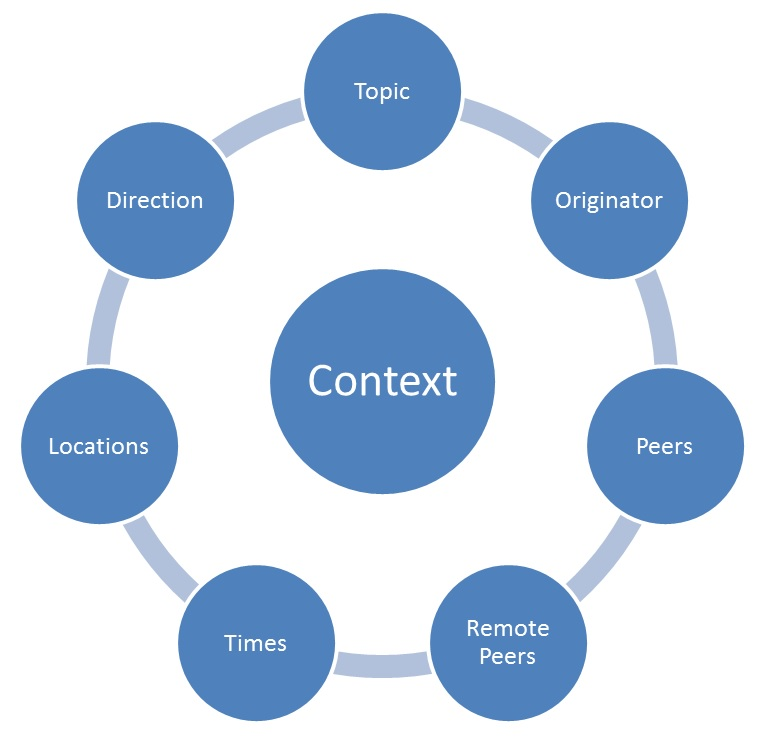
\includegraphics[width=\linewidth]{../Bilder/contextspace.jpg}
		\caption{Shark Context Space Modell}
		\label{fig:CSModel}
	\end{figure}
	
	Die einzelnen Elemente haben dabei folgende Bedeutung:
	\begin{itemize}
		\item \textbf{Topic:} Dies ist das Thema eines Kontextes. Es ist eine
		Beschreibung was der Kontext bedeutet.
		\newpage
		\item \textbf{Orginator:} Der Autor des beschriebenen Kontextes. Dies
		ist entweder der Ersteller sein oder der Autor der beiliegenden
		Informationen. Bei einem wissenschaftlichen Artikel wäre dies der Autor
		des besagten Artikels.
		\item \textbf{Peers:} Die Peers Dimension ist unterschiedlich 		
		interpretierbar. Zum einen kann es der Ersteller des Kontextes sein,
		was nicht dem Autor der beiliegenden Informationen entsprechen muss,
		zum anderen kann es	der Besitzer des Kontextes sein, wobei Besitzer hier
		je nach beiliegendem Fall anders interpretierbar ist. Im Allgemeinen
		kommt die Interpretation dieser Dimension auf den vorliegenden Fall an.
		\item \textbf{Remote Peers:} Dies sind die Peers an welche der Kontext
		gesendet werden soll.
		\item \textbf{Times:} Eine Zeitinformation, die je nach vorliegendem Fall
		anders interpretiert werden kann. Diese Dimension biete die Möglichkeit
		ein Zeitintervall anzugeben.
		\item \textbf{Locations:} Gibt einen Ort an. Auch hier ist je nach 
		vorliegenden Fall eine andere Interpretation möglich.
		\item \textbf{Direction:} Die Richtung der Kommunikation des Kontextes.
		Es ist möglich, Daten nur zu empfangen, sie nur zu senden, beide oder keine
		der genannten Aktionen durchzuführen.
	\end{itemize} 	
	
	Zu beachte ist, wenn von einem Kontext gesprochen wird, handelt es
	sich hierbei um eine Beschreibung einer Menge von Kontextpunkten. Diese
	Punkte haben den gleichen Aufbau wie in \autoref{fig:CSModel} gezeigt. Der 
	wesentliche Unterschied ist, dass ein Kontext eine Vielzahl von Inhalten,
	ausgenommen der Direction, besitzen kann. Währenddessen besitzt der
	Kontextpunkt nur je genau einen Inhalt. Beispielhaft beschreibt der
	Kontextpunkt nur das Thema Java, während der Kontext die Themen Java und C 
	beinhaltet kann. Die Dimensionen selbst werden als Kontextkoordinaten bezeichnet.
	Der Kontextpunkt vereint Koordinaten und Informationen. Der Kontext wiederum
	ist eine Möglichkeit, eine Menge an Kontextpunkten aus einer zugrundeliegenden
	Wissensbasis zu extrahieren.
	
	\subsubsection{Knowledge Base} 
	Die Knowledge Base, zu deutsch Wissensbasis, ist eine Sammlung von Wissen.
	Wissen ist dabei eine Menge an Informationen, die anhand von
	Kontextkoordinaten beschrieben sind. Die Vereinigung von Kontextkoordinaten
	und Informationen bilden einen Kontextpunkt.\\
	
	Die Wissensbasis bietet die Möglichkeit, Peers und Themen zu speichern, sowie
	die Themen in einer Taxonomie einzuordnen. Der für die zu entwickelnde
	Softwarekomponente wichtige Punkt ist aber die Möglichkeit, genannte
	Kontextpunkte in ihr zu speichern und anhand eines Kontextes zu extrahieren.
	Die Wissensbasis selbst kann hierbei ähnlich einer Datenbank angesehen werden.
	Ziel ist es, Teilbereiche, sprich eine bestimmte Menge an Daten, mit
	anderen Wissensbasen zu synchronisieren. Zu diesem Zweck gibt es bereits eine
	Implementierung, SyncKB genannt, auf der aufgebaut wird. \\
	
	Zusätzlich zu den genannten Eigenschaften gibt es die Möglichkeit Properties
	an der Wissensbasis zu speichern. Dies sind Name-Wert-Paare, wobei sowohl Name 
	als auch Wert eine Zeichenkette ist.
	
	\subsubsection{Knowledge Port} 
	Das wichtigste Objekt zur Kommunikation im Peer to Peer Netzwerk vom Shark
	Framework ist der KnowledgePort. Hierbei handelt es  sich um eine abstrakte
	Klasse,	welche die Implementierung von \emph{doExpose(SharkCS interest,
	KEPConnection kepConnection)} und \emph{doInsert(Knowledge knowledge,
	KEPConnection kepConnection)} erfordert. \\
	
	Die doExpose-Methode erhält ein Interesse in der Form eines SharkCS. Ist
	ein Interesse versandt worden, so wird sie als erstes aufgerufen. Ihre 
	generelle Aufgabe besteht darin zu ermitteln, ob das Interesse, das erhalten
	wurde, für den KnowledgePort von Relevanz ist. \\
	
	Die doInsert-Methode hingegen erhält ein Knowledge Objekt, welches echte
	Daten enthält. Es wird in der Regel gegen Ende der Kommunikation aufgerufen
	und soll die Daten in die Wissensbasis einfügen. \\
	
	Beide Methoden erhalten ein KEPConnection Objekt, mit dem sie Informationen 
	über den Sender bekommen können. Des Weiteren werden mithilfe dieses 
	Objektes Daten an die doExpose und doInsert-Methode anderer Peers gesendet.
	Dies erlaubt einen mehrfachen Datentausch. Ein Beispiel hierzu ist
	der Synchronisationsprozess der SychKB, der im nachfolgenden Abschnitt
	beschrieben wird und in \autoref{fig:SyncSeq} skizziert ist. \\
	
	Die Aussagen entsprechen hier dem Standardfall, wonach
	der Knowledge Port entworfen wurde. Die tatsächliche Implementierung und
	damit der Umgang mit dem SharkCS Objekt und dem Knowledge Objekt kann von jedem
	Entwickler selbst bestimmt werden. Einzig vorgeschrieben ist, dass zuerst
	ein Interesse versandt wird und Daten in der Form eines Knowledge Objektes
	gesendet werden.
	
	\subsubsection{SyncKB}
	\label{sec:SyncKB}
	
	Leider gibt es, abgesehen der JavaDoc Dokumentation, keine genaue
	Beschreibung der generellen Funktionsweise der SyncKB. Daher soll hier darauf
	eingegangen werden. Weitere Informationen
	können dem Quellcode selbst entnommen werden, der im Github vom SharkFW
	zu finden ist. \cite{SyncKB} \\
	
	Die SyncKB hält den Hauptteil ihrer Logik im SyncKP. Die eigentliche
	Synchronisation findet während des Kommunikationsprozesses statt und ist
	keine Eigenschaft der Wissensbasis selbst. Die einzelnen Elemente der SyncKB
	basieren hauptsächlich auf dem Entwurfsmuster Wrapper. So wurden den einzelnen
	Element zwei zusätzliche Informationen mitgegeben: 
	
	\begin{itemize}
		\item \textbf{Version:} Die aktuelle Version des Elements. Ein neu 
		erstelltes Element startet bei eins und bei jeder Änderung wird die
		Version um eins erhöht.
		\item \textbf{Zeitstempel:} Ein Zeitstempel der angibt, wann die letzte
		Änderung an dem Element vorgenommen wurde.
	\end{itemize} 
	
	Wie erwähnt, befindet sich der Großteil der Logik im SyncKP.
	\autoref{fig:SyncSeq} zeigt die ablaufende Kommunikation zwischen zwei
	Peers, die hier vereinfacht Alice und Bob genannt werden sollen.	
	
	\begin{figure}[H] 
		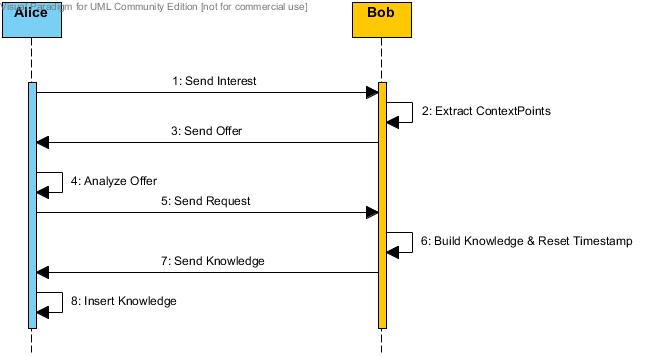
\includegraphics[width=\linewidth]{../Bilder/sync_seq.jpg}
		\caption{Kommunikation der SyncKB}
		\label{fig:SyncSeq}
	\end{figure}
	
	\begin{enumerate}
		\item \textbf{Interesse senden:} Der Prozess beginnt damit, dass Alice
		ihr Interesse zur Synchronisation verkündet. Das hierbei gesendete
		Interesse ist ein künstliches Interesse. Es wird vom SyncKP intern
		verwendet und dient lediglich als Datenhalter für diesen.
		\item \textbf{Kontextpunkte extrahieren:} Nachdem das Interesse an der
		Synchronisation Bob erreicht hat stellt dieser ein Angebot für Alice
		zusammen. Im linken Teil von \autoref{fig:SyncFlow} ist der
		Algorithmus dazu skizziert. Hierbei wird ausgenutzt, dass an jedem
		SyncContextPoint ein Zeitstempel der letzten Änderung gespeichert ist.
		Dieser wird mit dem Zeitpunkt des letzten Treffens mit dem Peer,
		das die Synchronisation anfordert, verglichen. Dazu ist an der
		Wissensbasis, per Property, eine Liste von Name-Wert-Paare gespeichert, 
		welche den Zeitpunkt des letzte Treffen mit einem Peer enthält.
		Genauer gesagt ist ein Peer jeweils einem Zeitstempel zugeordnet. Alle
		Kontextpunkte, deren letzte Änderung neuer ist als das letzte Treffe mit
		einem spezifischen Peer, hier Alice, werden angeboten.
		\item \textbf{Angebot senden:} Die extrahierten Kontextpunkte werden per
		Property am künstlichen Interesse gespeichert und Alice als Angebot
		zugesandt. Zu beachten	ist dabei, dass nur die Daten eines Kontextpunktes
		gesendet werden. Eventuelle Informationen, die diesem zugeordnet sind,
		werden nicht versandt.
		\item \textbf{Angebot analysieren:} Alice analysiert das Angebot, welches
		sie von Bob erhalten hat. Der Algorithmus ist ähnlich dem späteren Einfügen
		der Kontextpunkte und im rechten Teil von \autoref{fig:SyncFlow}
		skizziert. Alice wird alle Kontextpunkte von Bob anfragen, die sie
		nicht besitzt oder die bei Bob eine höhere Versionsnummer haben als
		bei ihr selbst.
		\item \textbf{Anfrage senden:} Abermals erfolgt ein Versand der
		Kontextpunkte per Property am künstlichen Interesse. Diesmal von Alice 
		zu Bob.
		\newpage
		\item \textbf{Wissen bauen und Zeitstempel setzen:} Nun extrahiert Bob die
		angefragten	Kontextpunkte aus seiner Wissensbasis und speichert sie in einem
		Knowledge Objekt. Zusätzlich werden	alle Themen und Peers,
		anhand des beim Erstellen des SyncKP übergebenen FragmentationParameter,
		dem Knowledge Objekt übergeben. Schließlich wird per Zeitstempel vermerkt,
		dass eine Kommunikation stattgefunden hat. Dies entspricht dem
		besprochenen letzten Treffen aus Punkt 2.
		\item \textbf{Wissen senden:} Das Knowledge Objekt wird nun an Alice
		gesendet.
		\item \textbf{Wissen in Wissensbasis einfügen:} Alice überprüft 
		die Kontextpunkte anschließend noch einmal anhand des im rechten Teil von
		\autoref{fig:SyncFlow} skizzierten Algorithmus und fügt diese dann in
		ihre Wissensbasis ein.
	\end{enumerate} 	
	
	\begin{figure}[H] 
		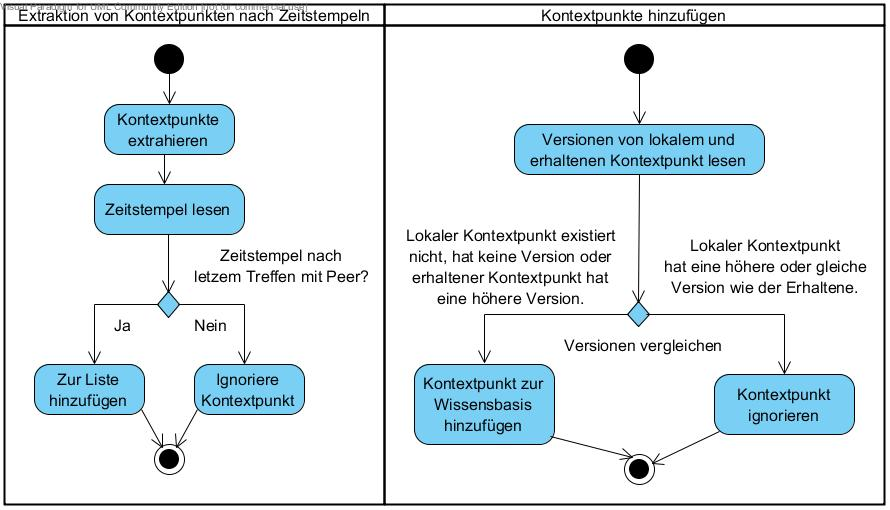
\includegraphics[width=\linewidth]{../Bilder/sync_flow.jpg}
		\caption{Algorithmus zum Extrahieren und Einfügen von Wissen der SyncKB}
		\label{fig:SyncFlow}
	\end{figure}
	
	Das System von Angebot und Anfrage wird verwendet, um das Datenvolumen während
	der Kommunikation möglichst gering zu halten. Wie erwähnt enthalten Angebot
	und Anfrage nur die nötigen Informationen zu den Kontextpunkten, wie
	Koordinaten, Zeitstempel und Version und nicht die mit dem Punkt verknüpften
	Informationen. Erst gegen Ende des Synchronisationsalgorithmus wird ein 
	Objekt mit den vollständiges Daten erstellt und versandt.
	
	\subsection{Datenstrukturen zur Darstellung von Beziehungen}
	\label{sec:datastruct}
	
	Wie in Abschnitt \ref{sec:requirements} beschrieben, soll es möglich sein
	Abhängigkeiten zwischen Räumen aufzustellen. Diese Abhängigkeiten stellen
	eine Beziehung zwischen Daten dar. Daher werden in diesem Abschnitt 
	Datenstrukturen besprochen, die eine solche Beziehung abbilden können.
	Dabei wird darauf eingegangen, wie die Daten und Beziehungen untereinander
	dargestellt sind. Weitergehende Erklärungen, wie mögliche Operationen, werden
	nur durch Links zu entsprechender Literatur gegeben.
	
	\subsubsection{Verkettete Listen}
	
	Verkettete Listen (beschrieben in \cite{FundData}, Kapitel 4) sind Listen,
	wo jedes Element Referenzen auf weitere Mitglieder der Liste enthält.
	Hier sollen die Einfach-Verketteten-Listen und die Zweifach-Verketten-Listen
	betrachtet werden.
	
	\paragraph{Einfach-Verkettete-Listen}\mbox{} \\
	
	Einfach-Verkettete-Listen besitzen eine Referenz auf ihren Nachfolger.
	Die Beziehung der einzelnen Elemente ist hierbei, dass jedes Element
	seinen Nachfolger kennt, nicht aber seinen Vorgänger. Die Beziehungen
	können also nur vorwärts verfolgt werden, das heißt, von einem Element
	zum Nachfolgenden, nicht aber von einem Element zum Vorherigen.
	\autoref{fig:single_linked_list} skizziert dieses und zeigt mögliche
	Operation an einer verketteten Liste auf. Weitere Informationen können
	den Erklärungen unter \cite{SLList} entnommen werden.
	
	\begin{figure}[H] 
		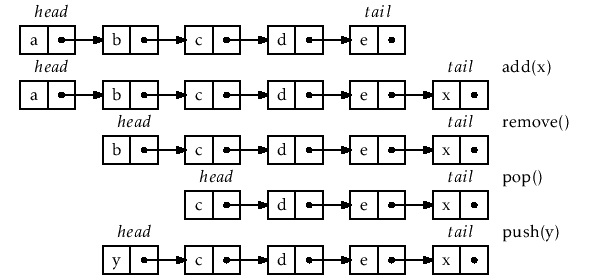
\includegraphics[width=\linewidth]{../Bilder/single_linked_list.jpg}
		\caption
		{
			Aufbau und Operation von Einfach-Verkettete-Listen.
			Quelle: \cite{SLList}
		}
		\label{fig:single_linked_list}
	\end{figure}	
	
	\paragraph{Zweifach-Verkettete-Listen}\mbox{} \\
	
	Zweifach-Verkettete-Listen besitzen, gegenüber Einfach-Verkettete-Listen,
	eine Referenz auf Vorgänger und Nachfolger. Die Beziehung der einzelnen
	Elemente ist also, dass jedes Element seinen Vorgänger und Nachfolger
	kennt. Somit kann die Liste vorwärts, von Element zum nachfolgenden
	Element, als auch rückwärts, vom Element zum vorhergehenden Element,
	verfolgt werden. \autoref{fig:double_linked_list} skizziert dieses.
	Weitere Informationen können den Erklärungen unter \cite{DLList} entnommen
	werden.
	
	\begin{figure}[H] 
		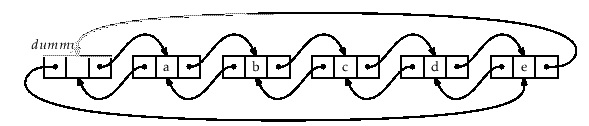
\includegraphics[width=\linewidth]{../Bilder/double_linked_list.jpg}
		\caption
		{
			Aufbau von Zweifach-Verkette-Listen.
			Quelle: \cite{DLList}
		}
		\label{fig:double_linked_list}
	\end{figure}	
	
	\subsubsection{Bäume}
		
	Bäume (\cite{FundData}, Kapitel 4) bestehen aus einem Wurzelknoten
	und weiteren Knoten, die von diesem ausgehen. Hierbei besteht eine Vater-Kind
	Beziehung zwischen diesen. Die Wurzel hat die besondere Eigenschaft, dass
	sie keinen Vater besitzt. Knoten, die keine Kinder besitzen, werden Blätter
	genannt. Ein Element kann hier also mit beliebig vielen Unterelementen, seinen
	Kindern, in Beziehung stehen. Hingegen kann ein Element von nur einem anderen
	Element abstammen. \autoref{fig:tree} skizziert ein Beispiel
	dieser Datenstruktur.
	
	\begin{figure}[H] 
		\centerline{
			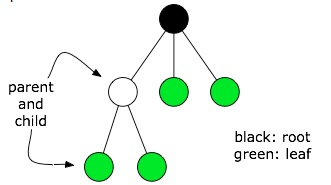
\includegraphics{../Bilder/tree.jpg}
		}
		\caption
		{
			Aufbau eines Baums.
			Quelle: \cite{Trees}
		}
		\label{fig:tree}
	\end{figure}
	
	\subsubsection{Graphen}
	
	Graphen (siehe \cite{FundData}, Kapitel 6) bilden ein Netz von Daten. Dabei
	kann von jedem Element eine Beziehung zu einem anderen ausgehen. Gegenüber
	Bäumen besitzen sie keine Wurzel, welche den Anfang darstellt. Zudem ist die
	Anzahl an Beziehungen nicht festgelegt. Ein Element besitzt eine Vielzahl von
	Beziehungen. Gerichtete Graphen geben dieser Beziehung eine Richtung.
	Somit kann allerdings nur angegeben werden, von welchem Element man zu welchen
	gelangt und gegebenenfalls nicht mehr zurück. Dies ist ähnlicher dem 
	Nachfolger Link in einer verketteten Liste und stellt nicht,
	wie beim Baum, eine Vater-Kind Beziehung dar. Des Weiteren besteht die
	Möglichkeit gewichteten Graphen Metadaten, wie die Kosten für einen
	Übergang von Element A zu Element B, mitzugeben. Dennoch bleibt
	die Art, wie zwei Elemente im Detail zueinander in Beziehung stehen,	
	unbeschrieben. \autoref{fig:graph} skizziert das Modell eines gerichteten
	Graphen. Die Pfeile stellen dabei die Übergänge zwischen den Elementen dar.
	Weitere Erklärungen können unter \cite{Graph} gefunden werden. 

	\begin{figure}[H] 
		\centerline{
			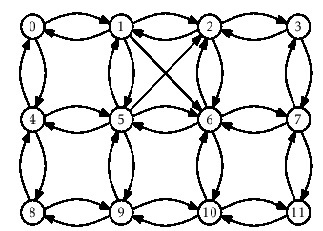
\includegraphics[scale=0.8]{../Bilder/graph.jpg}
		}
		\caption{Aufbau eines Graphen. Quelle: \cite{Graph}}
		\label{fig:graph}
	\end{figure}
	
	\subsubsection{Entity Relationship Modell}
	
	Das Entity Relationship Modell, beschrieben in \cite{EntRel}, ist weniger
	eine Datenstruktur, als ein Modell zur Beschreibung von Zusammenhängen zwischen
	Daten, bekannt aus relationalen Datenbanksystemen. Damit beschreibt es aber
	auch eine Beziehung und kann somit als Grundlage herangezogen werden. Die
	Beziehungen basieren darauf, dass jedes Element einen eindeutigen 
	Primärschlüssel besitzt. Datensätzen, die mit anderen Datensätze, in Beziehung 
	stehen, besitzen einen Fremdschlüssel, welcher identisch zum Primärschlüssel
	des Datensatzes ist, mit dem sie in Beziehung stehen. \autoref{fig:ent_rel}
	zeigt eine vereinfachte Skizze dieser Beziehung auf. Anders als die Abbildung
	erscheinen lässt, sind diese Schlüssel nicht an einen Datentypen gebunden. Auch
	kann ein Schlüssel mehrere Daten eines Datensatzes umfassen. Die Trennung
	in Primärschlüssel und Fremdschlüssel erlaubt auch die Art der Beziehung zu
	interpretieren. Beispielsweise kann dies eine Vater-Kind Beziehung darstellen.
	Das Modell ist aber nicht an diese Interpretation gebunden.
	
	\begin{figure}[H] 
		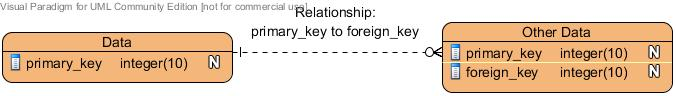
\includegraphics[width=\linewidth]{../Bilder/ent_rel.jpg}
		\caption{Vereinfachte Skizze des Entity Relationship Modell}
		\label{fig:ent_rel}
	\end{figure}	
	
	\subsection{Aufbau von Social Media Formaten}	
	\label{sec:social}
	
	In diesem Abschnitt soll der Aufbau einer Reihe von Social Media Formaten
	beschrieben werden. Social Media Formate sind dabei Anwendungen, die
	den Kontakt mit anderen Menschen fördern. Die Verknüpfung der einzelnen
	Informationen und Daten miteinander soll hierbei von besonderem Interesse sein,
	da sie die Abhängigkeiten aus Abschnitt \ref{sec:requirements} darstellen.
	
	\subsubsection{Chat}	
	
	Chats sind einer der einfachsten Möglichkeiten der Kommunikation. Abbildung
	\ref{fig:chat} zeigt den Aufbau eines Chat im Programm Skype.
	
	\begin{figure}[H] 
		\centerline{
			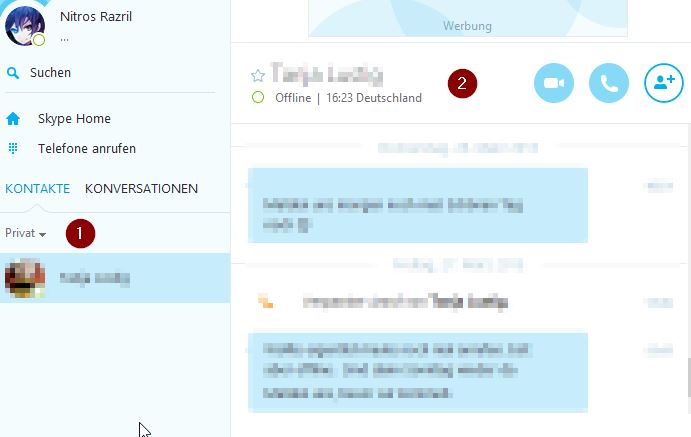
\includegraphics[scale=0.58]{../Bilder/chat.jpg}
		}
		\caption{Aufbau Chat in Skype. \cite{chat}}
		\label{fig:chat}
	\end{figure}		
	
	Die Aufteilung erfolgt hier in erster Ebene (1) in Gruppen. In zweiter Ebene (2)
	ist der eigentliche Chat. Ein Chat besitzt eine Vielzahl von Daten. Ein
	Eintrag enthält beispielsweise einen Zeitstempel, Text und Autor der
	Nachricht. Der Chat selbst erscheint identifizierbar durch einen nicht
	sichtbaren Identifikator, da Elemente wie Teilnehmer geändert werden können
	und der Chat trotzdem auffindbar ist. Vereinfacht kann man sagen, dass ein
	Chat ein einzelner Raum von Informationen ist, der auf eine bestimmte Art
	durch einen oder mehrere Identifikatoren dargestellt wurde.
	
	\subsubsection{Forum}	
	
	Ein Forum ist gegenüber einem Chat meist komplexer und lässt sich in mehrere
	Ebenen einteilen. Als Beispiel soll das	Burning Board der WoltLab GmbH
	herangezogen werden \cite{BB}. In den folgende Abbildungen
	\ref{fig:forumstruc001}, \ref{fig:forumstruc002} und \ref{fig:forumstruc003}
	ist der strukturelle Aufbau eines Forums zu sehen.
	
	\begin{figure}[H] 
		\centerline{
			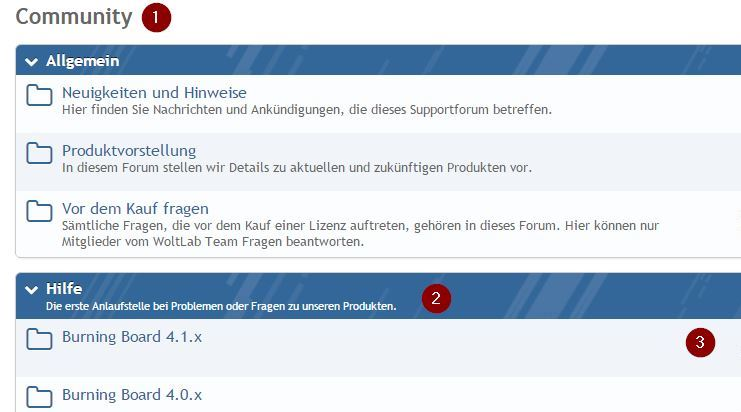
\includegraphics[scale=0.65]{../Bilder/forumstruc001.jpg}
		}
		\caption{Forumstruktur: Oberste Ebene. Quelle: \cite{BB}}
		\label{fig:forumstruc001}
	\end{figure}	
	
	\newpage
	\autoref{fig:forumstruc001} zeigt die oberste Ebene eines Forums. Man sieht
	eine Baumstruktur mit einer Wurzel (1). Von diesem Baum gehen Äste (2) aus,
	von welchem wiederum weitere Äste (3) abzweigen können.
	
	\begin{figure}[H] 
		\centerline{
			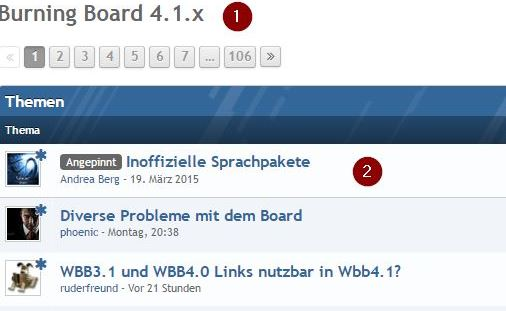
\includegraphics[scale=0.73]{../Bilder/forumstruc002.jpg}
		}
		\caption{Forumstruktur: Thread-Sammlung Ebene. Quelle: \cite{BB}}
		\label{fig:forumstruc002}
	\end{figure}	
	
	\autoref{fig:forumstruc002} zeigt die Ebene in der die Threads mit den
	Inhalten zu finden sind. Man sieht, dass es sich hierbei um einen Knoten (1)
	in der zuvor erwähnten Baumstruktur handelt. Die einzelnen Threads (2) stellen
	dabei die Blätter des Baumes dar.
		
	\begin{figure}[H] 
		\centerline{
			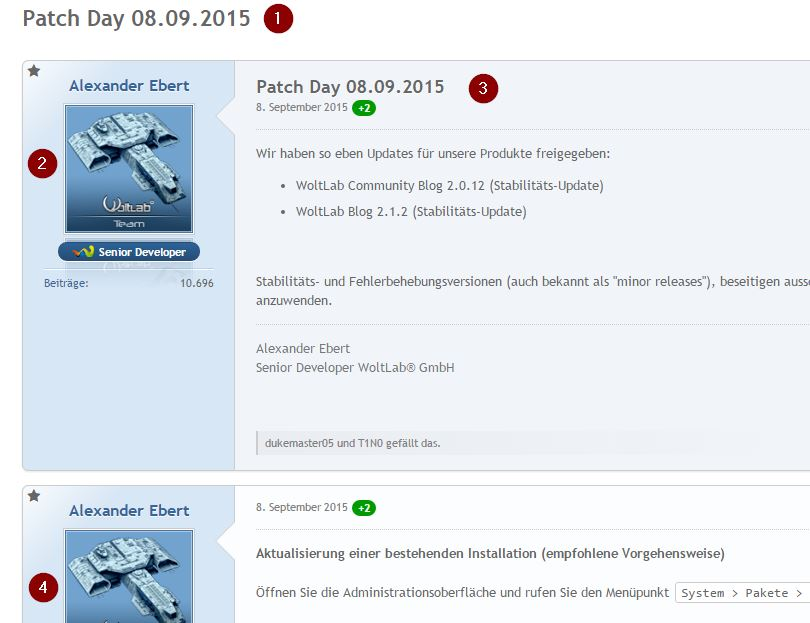
\includegraphics[scale=0.6]{../Bilder/forumstruc003.jpg}
		}
		\caption{Forumstruktur: Thread Ebene. Quelle: \cite{BB}}
		\label{fig:forumstruc003}
	\end{figure}	
	
	\autoref{fig:forumstruc003} zeigt einen Thread in einem Forum. Dieser ist
	ein Blatt (1) in der Baumstruktur. Ähnlich wie der Chat ist ein Thread ein
	Raum von Daten. Die einzelnen Einträge (3, 4) besitzen dabei  ähnliche Daten
	zum Chat. Beispiele für diese Daten sind: Zeitstempel, Text und Autor (2). \\
	
	Trotz des unterschiedlichen Layouts der grafischen Oberfläche besitzen
	Threads und Chat eine Vielzahl von Gemeinsamkeiten in ihrem Aufbau. Der
	größte Unterschied ist, dass Foren sich einer Baumstruktur bedienen, um
	die einzelnen Räume von Daten unter- oder oberhalb von anderen Räume 
	einzuordnen. Dies kann
	als Vater-Kind Beziehung eines Baumes gesehen werden, wobei hier nur die Blätter
	Daten enthalten. Andere Knoten dienen lediglich einer Ordnung der Daten und 
	der Eingruppierung dieser in einen definierten Bereich. Jeder Knoten kann
	aber potenziell Threads enthalten.
	
	\subsubsection{Dateisysteme und Versionsverwaltung Software}	
	
	Es mag auf den ersten Blick nicht so erscheinen, aber auch Dateien aus
	dem Dateisystem können für soziale Kontakte genutzt werden. Ein einfaches
	Beispiel hierfür ist die Existenz der vielen Image-Hoster. Auch 
	Facebook und Instagram erlauben den Austausch von Bildern. \\
	
	In diesem Sinne kann auch Versionsverwaltung Software wie Git oder SVN als
	eine Art des sozialen Kontaktes gesehen werden. In einem Online Artikel der
	t3n \cite{articleGitHub} wird beschrieben, dass man immer mehr auf den
	webbasiertern Filehosting-Dienst für Software-Entwicklungsprojekte GitHub
	\cite{gitHub} stößt, der auf Git basiert. Mit seiner Vielzahl an Projekten
	der unterschiedlichsten Programmiersprachen kann GitHub als soziale Plattform
	für Softwareentwickler gesehen werden. \\
	
	Aus diesem Grund soll der Austausch von Teilen des Dateisystems über solche 
	Versionsverwaltung Software auch Betrachtung finden. Die eigentliche
	Versionierung wird dabei vernachlässigt. \autoref{fig:filesytsem}
	zeigt den allgemeinen Aufbau von Dateisystemen für unterschiedliche
	Betriebssysteme.
	
	\begin{figure}[H] 
		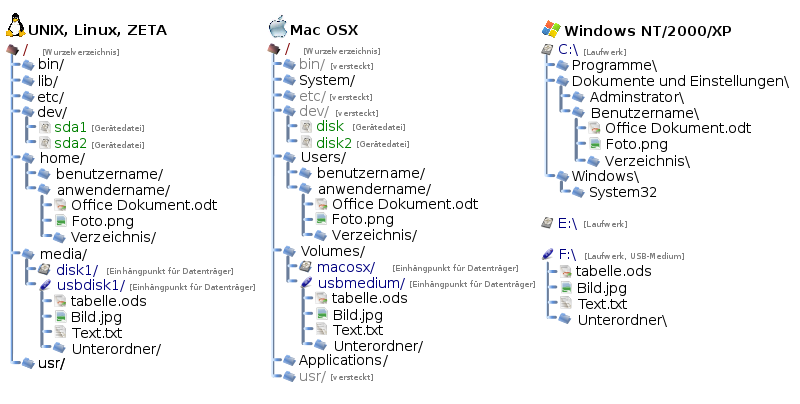
\includegraphics[width=\linewidth]{../Bilder/filesystem.png}
		\caption{
			Illustration über den Vergleich von Dateisystem-Bäumen.
			Quelle: \cite{filesytsem}
		}
		\label{fig:filesytsem}
	\end{figure}
	
	\newpage
	Zu sehen ist, das identisch zum Forum eine Baumstruktur die Grundlage von
	Dateisystemen ist. Hier enthalten nur die Blätter die eigentlichen Daten und die
	anderen Knoten dienen lediglich der Eingruppierung von Daten. Die Blätter selbst
	können als ein einzelnes Element, bestehend aus Bytes und angereichert mit
	Metadaten, gesehen werden. Dies unterscheidet sich zum Chat oder Forum, wo ein
	Blatt ein beschriebener Raum von Daten ist. 
	
	\subsection{Tags zur Beschreibung von Inhalten}
	\label{sec:tags}
	
	Das sogenannte Tagging von Inhalten ist spätestens seit den Twitter Hashtags
	bekannt. Es kommt in vielen Formen zum Einsatz. \autoref{fig:tags} zeigt es
	auf der Frage- und Antwortplattform stackoverflow.
	
	\begin{figure}[H] 
		\centerline{
			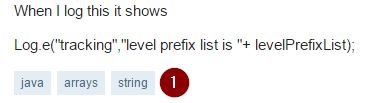
\includegraphics[scale=0.95]{../Bilder/tags.jpg}
		}
		\caption{
			Illustration von Tags an einer Frage in stackoverflow.
			Quelle: \cite{stackoverflow}
		}
		\label{fig:tags}
	\end{figure}
	
	Die Tags (1) dienen dabei der Eingruppierung der Frage. Beim Klick auf eines
	der Tags gelangt man zu einer Liste von Fragen, die das gleiche Tag tragen. \\
	
	Was ist der Grund zur Nutzung von Tags? Oded Nov, Mor Naaman und Chen Ye
	beschreiben es in ihrer Publikation What Drives Content Tagging: The Case of
	Photos on Flickr \cite{CaseTag} als eine Möglichkeit, Inhalte mit Metadaten
	in der Form von Schlüsselwörtern anzureichern. Der Nutzer bedient sich der Tags, 
	damit seine Inhalte besser von anderen gefunden werden. Dies tut er, um seine
	soziale	Präsenz zu erweitern. Scott A. Golder und Bernardo A. Huberman
	beschreiben Tags in The Structure of Collaborative Tagging 
	Systems \cite{CollTag} als eine	Möglichkeit, Inhalte für zukünftige Navigation,
	Filterung und Suche zu organisieren. Des Weiteren wird ausgeführt, dass Tags
	Informationen zu folgenden Aspekten geben können:
	
	\begin{itemize}
		\item Über was oder wen ist der Inhalt?
		\item Was für ein Inhalt ist es, ein Buch oder ein Artikel
		in einer Zeitschrift?
		\item Wem gehört der Inhalt?
		\item Einordnung in eine Kategorie
		\item Bewertung des Inhaltes, wie lustig oder unheimlich.
		\item Selbstreferenzen, wie \emph{mystuff} oder \emph{mycomments},
		um die Relation zu einem selbst darzustellen.
		\item Organisieren von Aufgaben, beispielsweise Tags wie \emph{toread} oder
		\emph{jobsearch}.
	\end{itemize}
	
	Im Allgemeinem sind Tags eine Möglichkeit Inhalte zu organisieren. Sie können
	auch als eine Beschreibung des Inhalts gesehen werden, wobei diese Beschreibung
	vielen Zwecken dienen kann.
		
	\newpage
	
	\section{Konzeption}	
	
	In diesem Abschnitt wird die Konzeption der geplanten Softwarekomponente
	besprochen. Basierend auf den Grundlagen des vorherigen Kapitels wird eine
	Auswahl getroffen und Techniken zur Implementieren gewählt.
	
	\subsection{Serialisierung}
	\label{sec:konz_serialisierung}
	
	Eine der Anforderungen aus dem Abschnitt \ref{sec:requirements} war Persistenz.
	Es sollte möglich, sein eine Beschreibung eines Raumes zu speichern um sie später
	wieder abrufen zu können. Zu diesem Zweck macht es Sinn das Feature des Setzen
	von Properties an einer Wissensbasis zu nutzen. Auf diesem Weg kann je 
	Wissensbasis eine Liste von Beschreibungen gespeichert werden. Insbesondere
	kann dies als Zuordnung dieser Beschreibungen zur entsprechenden Wissensbasis
	gesehen werden. \\
	
	Dazu benötigen wir eine Technik, welche die Serialisierung eines Objektes einer
	Programmiersprache, in diesem Fall Java, in eine Zeichenkette ermöglicht. Um
	die Anforderung der Wartbarkeit zu gewährleisten soll hier ein menschlich
	lesbares Format gewählt werden, dass von den meisten Entwicklern verstanden
	wird. XML und JSON erfüllen diese Anforderungen. Zum Vergleich sollen die
	Ergebnisse aus der Fallstudie \cite{XmlJson} zurate gezogen werden.
	Diese sind in den folgenden Abbildungen dargestellt.
	
	\begin{figure}[H] 
		\centerline{
			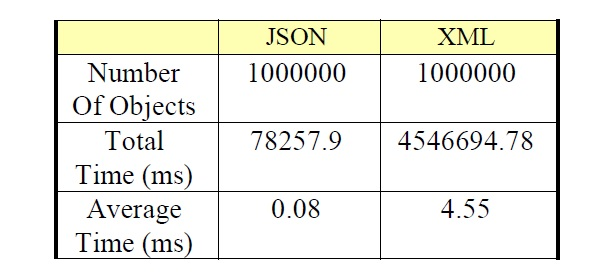
\includegraphics[scale=0.78]{../Bilder/xml_json_time_sen1.jpg}
		}
		\caption{Scenario 1 JSON vs. XML Timing. Quelle: \cite{XmlJson}}
		\label{fig:xml_json_time_sen1}
	\end{figure}
	
	\begin{figure}[H] 
		\centerline{
			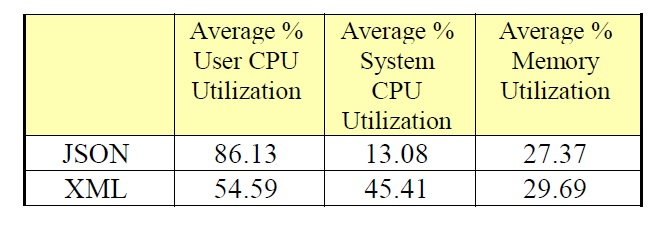
\includegraphics[scale=0.78]{../Bilder/xml_json_mem_sen1.jpg}
		}
		\caption{Scenario 1 JSON vs. XML CPU/Mem. Quelle: \cite{XmlJson}}
		\label{fig:xml_json_mem_sen1}
	\end{figure}
	
	\newpage
	
	Die Abbildungen \ref{fig:xml_json_time_sen1} und \ref{fig:xml_json_mem_sen1}
	zeigen den ersten Fall der Fallstudie. Hier wurde eine große Menge an Daten
	über einen Kommunikationskanal gesendet. Es ist klar ersichtlich, dass JSON
	in den Bereichen Timing und CPU/Memory eine bessere Qualität aufzeigt. Einzig
	bei der Nutzung der CPU des Nutzers zeigt XML bessere Werte auf.
	
	\begin{figure}[H] 
		\centerline{
			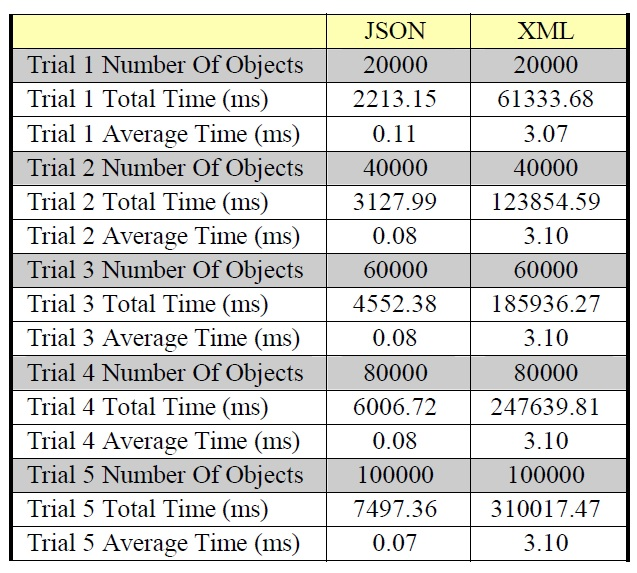
\includegraphics[scale=0.8]{../Bilder/xml_json_time_sen2.jpg}
		}
		\caption{Scenario 2 JSON Vs XML Timing. Quelle: \cite{XmlJson}}
		\label{fig:xml_json_time_sen2}
	\end{figure}
	
	\begin{figure}[H] 
		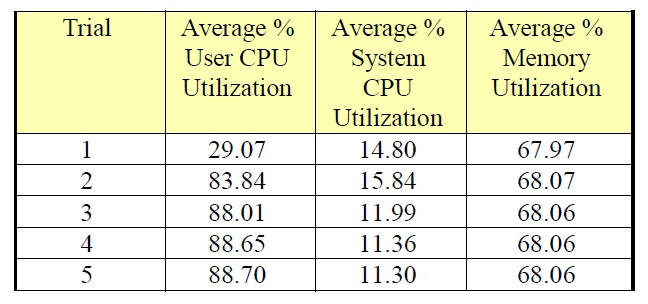
\includegraphics[width=\linewidth]{../Bilder/json_mem_sen2.jpg}
		\caption{Scenario 2 JSON CPU/Mem. Quelle: \cite{XmlJson}}
		\label{fig:json_mem_sen2}
	\end{figure}
	
	\begin{figure}[H] 
		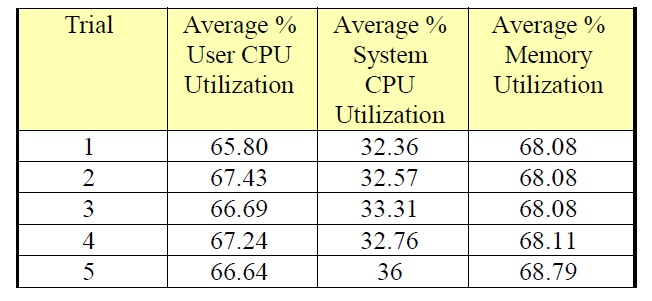
\includegraphics[width=\linewidth]{../Bilder/xml_mem_sen2.jpg}
		\caption{Scenario 2 XML CPU/Mem. Quelle: \cite{XmlJson}}
		\label{fig:xml_mem_sen2}
	\end{figure}
	
	Die Abbildungen \ref{fig:xml_json_time_sen2}, \ref{fig:json_mem_sen2}
	und \ref{fig:xml_mem_sen2} zeigen den zweiten Fall der Fallstudie. Hier
	wurden mehrfach hintereinander kleine Datensätze übertragen anstatt alle
	Datenobjekte in einer Übertragung zu senden. Auch hier zeigt sich, dass
	JSON im Allgemeinen bessere Werte liefert. Nur bei der Nutzung der CPU des
	Nutzers zeigt XML, wie im ersten Fall, bessere Werte auf. \\
	 
	Mit den vorliegenden Daten würde die Wahl normalerweise auf JSON fallen.
	Allerdings handelt es sich bei der zu entwickelnden Softwarekomponente um
	einen Teil eines Frameworks. Das erfordert eine gesonderte Sichtweise. 
	
	\begin{itemize}
		\item \textbf{Abhängigkeiten:} Umgangssprachlich gibt es den Begriff der
		"Jar-Hölle". Dieser beschreibt, dass Frameworks ihre Abhängigkeiten in der
		Form von Jar-Archiven mitbringen und dadurch die Möglichkeit besteht, diese
		mehrfach in einem Projekt zu haben. Das erhöht den Speicherbedarf einer
		Applikation unnötig. Auf der anderen Seite kann es passieren, dass keine
		Abhängigkeiten mitgebracht werden und von Entwickler eigenständig
		hinzugefügt werden müssen. Dies erfordert einen ausdrücklichen Hinweis in
		der Dokumentation, wobei nicht sichergestellt werden kann, ob dieser
		gelesen	wird. Zwar kann dies durch das Nutzen eines Tools wie Maven
		verhindert werden, allerdings nutzt das Shark Framework dieses Tool nicht.
		Insofern ist interessant, dass Java von Hause aus durch Java Architecture 
		for XML Binding, kurz JAXB, XML unterstützt.
		JSON hingegen erfordert das Einbinden eines zusätzlichen Frameworks.
		\item \textbf{Einheitlichkeit:} Das Shark Frameworks benutzt bereits eine
		XML Repräsentation an vielen Stellen. Ein Mix von XML und JSON bei der
		Benutzung kann durchaus verwirrend für Entwickler sein, besonders
		im Bezug auf die Weiterentwicklung des Frameworks. Die zur Zeit proprietäre
		XML Serialisierung sollte einfacher auf das im Java Development Kit
		enthaltene JAXB umzustellen sein als auf ein externes Framework für JSON,
		sofern dies bei zukünftigen Refactoring Aktionen geplant ist.
		\newpage
		\item \textbf{XML Schema:} XML bietet die Möglichkeit, den
		Aufbau der XML Datei über XML-Shema und DDTs zu beschreiben. Dadurch
		können XML-Parser erkennen, ob ein XML-Dokument valide ist. JSON fehlt
		diese Möglichkeit. Im Sinne der Wartbarkeit ist dies ein Feature, dass
		zukünftig an Bedeutung gewinnen könnte. Speziell, da das Shark Framework
		aus einer Vielzahl komplexer Objekte besteht, die beim Datenaustausch
		versandt werden.
		\item \textbf{sun.misc.Unsafe:} Wie ein Artikel auf JAXenter \cite{unsafe}
		beschreibt, plante Oracle ursprünglich für Java 9 die Entfernung von
		sun.misc.Unsafe. Diese wird dennoch von vielen Frameworks genutzt. Da
		JAXB Bestandteil des normalen Java Development Kit von Oracle ist, sind
		hier, gegenüber der Verwendung von Frameworks Dritter, keine Probleme zu
		erwarten.	
	\end{itemize} 	
	
	Wegen dieser Aspekte, insbesondere dem Punkt Abhängigkeiten, soll hier die
	Darstellung in XML erfolgen.
	
	\subsection{Unterscheidung in Beschreibung und Synchronisation}
	
	Per Konzept wird im Rahmen dieser Arbeit in Beschreibung und Synchronisation
	unterschieden. Die Synchronisation dient zur Darstellung eines Datenbereiches
	und ist unabhängig vom Algorithmus zum Synchronisieren. Die Synchronisation
	hingegen baut auf der Beschreibung auf. Sie  umfasst ebenfalls den Ablauf
	der Kommunikation zwischen zwei oder mehr Peers. Dies ermöglicht eine modulare
	Unterscheidung. \\
	
	Die Beschreibung dient dem Extrahieren von Daten. Wie mit diesen
	Daten umgegangen wird ist nicht festgelegt. Währenddessen enthält die
	Synchronisation die eigentliche Logik zum Ausführen der partiellen
	Synchronisation. 	
	
	\subsection{Ein Nachschlagewerk für Datenbereiche}
	
	Wie in Abschnitt \ref{sec:tags} beschrieben, eignen sich Tags zum organisieren,
	filtern und suchen von Inhalten. Die Datenbereiche, die beschrieben werden
	sollen, können als Inhalte aufgefasst werden. Wenn es also gelingt, diese Inhalte
	mittels eines Kontextes zu beschreiben, sind sie einfach wiederzufinden.
	Der Kontext ersetzt dabei das Tag. Gelingt es ebenfalls diese Beschreibungen in
	Beziehungen untereinander zu setzen, kann ein Nachschlagewerk für
	Datenbereiche aufgebaut werden. So könnten sich unter dem Schlagwort
	Programmiersprachen die Schlagwörter Java und C befinden. 
	Je nach Suchalgorithmus wären so Abhängigkeiten auffindbar
	und Datenbereiche könnten entsprechend erkannt werden. Die Idee ist hierbei
	ähnlich der Themen und Peer Taxonomie, welche bereits in einer Wissensbasis
	existieren. Allerdings ist die Idee hier auf einen Kontext bezogen.
	
	\subsection{Darstellung eines Datenbereiches über einen Deskriptor}
	
	In diesem Abschnitt wird besprochen, wie ein Datenbereich dargestellt werden
	soll. Dazu betrachten wir die Datenstrukturen aus Abschnitt
	\ref{sec:datastruct} und den Aufbau von Social Media Formaten aus Abschnitt
	\ref{sec:social}. Interessant dabei ist, inwiefern sie zur Implementierung der
	Beschreibung des Datenbereiches genutzt werden können, so dass eine Struktur
	ähnlich der Social Media Formate erreicht werden kann. Auch inwiefern
	diese zu XML serialisiert werden können, findet dabei Betrachtung. Zu diesem
	Zweck wird ein Objekt zur Beschreibung eines Datenbereiches eingeführt: Der
	Deskriptor. 
	
	\subsubsection{Analyse der Datenstrukturen}
	
	Im folgenden wird auf die Analyse der in  Abschnitt \ref{sec:datastruct}
	beschriebenen Datenstrukturen in Bezug auf die in Abschnitt \ref{sec:social}
	genannten Social Media Formate eingegangen.
	
	\paragraph{Verkettete-Listen}\mbox{} \\
	
	Verkettete-Listen erlauben das Darstellen einer Vater-Kind Beziehung. Bei
	Zweifach-Verketteten-Listen könnte hier vorwärts und rückwärts nach Elementen
	gesucht werden. Serialisiert wären sie in XML durch eine einfache Liste,
	mit einer vorgegebenen festen Reihenfolge. Das bedeutet, jedes Element müsste
	im XML in der Reihenfolge erscheinen, in der es in der Liste gespeichert ist. \\
	
	Verkettete-Listen haben allerdings den Nachteil, dass je nur ein
	Vorgänger und Nachfolger definiert werden kann. Daher eignen sie sich weniger
	für die Darstellung der Baumstruktur eines Forums oder eines Teil des
	Dateisystems. 	
	
	\paragraph{Bäume}\mbox{} \\
	
	Die meisten der besprochenen Social Media Formate haben von Grund auf eine
	Baumstruktur. Daher lassen sie sich ohne größere Probleme auch als eine
	Solche darstellen. Da XML ebenfalls eine Baumstruktur besitzt, über
	die Tags als Subtags anderer Tags dargestellt werden können, ist auch
	die Serialisierung in diesem Format kein Problem. \\
	
	Problematisch hingegen ist die Tatsache, dass in der Programmiersprache 
	Java, in welcher die Softwarekomponente geschrieben wird, keine vorgefertigten
	Datenstrukturen für Bäume existieren.
	
	\paragraph{Graphen}\mbox{} \\
	
	Bäume sind prinzipiell eine besondere Art von Graphen. Daher lassen sich
	die Social Media Formate auch als diese darstellen. Problematisch
	könnte hierbei sein, die Wege von einem Knoten zu einem anderen zu
	serialisieren. Dabei kann es sehr einfach zu doppelter Datenhaltung kommen. \\
	
	Allgemein wären Graphen zu weit gefasst. Kosten für die Wege sind nicht
	ausschlaggebend für die Beschreibung einer Beziehung. Auch kann angenommen
	werden, dass man von einem Vater immer zu seinen Kindern kommt und das ein Kind
	immer seinen Vater kennt. Bäume sind für diesen Aspekt ausreichend, besonders da
	sie einen Startpunkt, die Wurzel, besitzen.
	
	\paragraph{Entity Relationship Modell}\mbox{} \\
	
	Auch wenn das Entity Relationship Modell eher ein Modell als
	eine Datenstruktur darstellt, ist ein Element in diesem trotzdem
	durch einen Primärschlüssel eindeutig beschrieben.
	Eine Beziehung zu einem Anderen lässt sich hier einfach durch einen
	Fremdschlüssel erreichen. Dies ermöglicht die Flexibilität, dass ein Element
	sehr leicht mehre Kinder und Väter haben kann, auch als 1:1, 1:N. N:M Beziehung
	aus Datenbanksystemen bekannt. Viele Elemente der Social Media Formaten sind
	durch einen Identifikator identifizierbar. Beispielsweise kann ein Thread eines
	Forums einen numerischen Identifikator besitzen. Dieser kann bei der
	URL Generierung	genutzt werden, um eine eindeutige URL zu erzeugen. Daher sollte
	es auch möglich sein, diesen Identifikator zur Identifikation eines Raumes zu
	nutzen. Auf übergeordnete Elemente kann mittels des Fremdschlüssels ebenfalls
	einfach verwiesen werden. Beziehungen sind daher, entsprechend des Namens des
	Modells, leicht abzubilden.	Wenn es sich bei besagtem Identifikator um einen
	primitiven Datentypen oder eine Zeichenkette handelt, so ist die
	Serialisierung nur ein zusätzliches Tag im XML mit ihm als Inhalt. \\
	
	Problematisch ist, dass die einzelnen Beziehungen programmatisch 
	zusammengesetzt werden müssen. Im Rahmen dieser Arbeit existiert keine
	relationale	Datenbank mit einem Datenbanksystem, welches diese übernehmen
	könnte.
	
	\paragraph{Auswertung}\mbox{} \\
	
	Da die beschriebenen Social Media Formate bereits eine baumartige Struktur
	aufweisen, ist es sinnvoll, auch die Datenstruktur eines Baumes zu nutzen. Um
	die eigentlichen Vater-Kind Beziehungen darzustellen, kann das Prinzip des
	Entity Relationship Modell aus Datenbanken verwendet werden. Dies ermöglicht
	einen Identifikator für einen Raum zu definieren, anhand dessen er wieder
	auffindbar ist. Das Ganze kann als eine Liste serialisiert werden, wobei
	jeder Identifikator nur einmal vorkommt.
	
	\subsubsection{Beschreibung eines Datenbereiches durch einen Deskriptor}
	\label{sec:desk}
	
	Nach der Analyse aus dem vorhergehenden Abschnitt soll nun festgelegt werden
	mit welchen Parametern ein Datenbereich beschrieben wird.
	\autoref{fig:descriptor} zeigt den Aufbau des beschreibenden Elements, dem
	Deskriptor.
	
	\begin{figure}[H] 
		\centerline{
			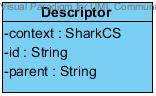
\includegraphics{../Bilder/descriptor.jpg}
		}
		\caption{Konzeption eines Deskriptor}
		\label{fig:descriptor}
	\end{figure}
	
	Dieses Element soll Deskriptor genannt werden. Es besitzt die folgenden
	Parameter:
	
	\begin{itemize}
		\item \textbf{Kontext (context):} Der Kontext ist der Kern des Deskriptors.
		Er bestimmt, welche Kontextpunkte durch ihn aus der Wissensbasis extrahiert
		werden können. Dabei ist es allerdings auch möglich ihm keine Bedeutung 
		zuzuordnen. Dies macht Sinn, wenn der Deskriptor nur zur Beschreibung einer
		Beziehung benutzt wird, beispielsweise eines Ordners in einem Dateisystem.
		Dabei ist dann nur interessant, welche Kinder dieser besitzt, nicht aber
		die Kontextpunkte, die er beschreibt. So ein Deskriptor soll leerer
		Deskriptor genannt werden.
		\item \textbf{Identifikator (id):} Der Identifikator ist ein Teil des
		Paares, welche die Vater-Kind Beziehung ermöglicht. Des Weiteren
		ermöglicht er das Wiederauffinden eines bestimmten Deskriptors aus einer
		Liste von Deskriptoren.
		\item \textbf{Vater (parent):} Der Vater ist der andere Teil des Paares,
		welche die Vater-Kind Beziehung ermöglicht. Er erlaubt das Auffinden des
		Vaters eines Deskriptors. Ebenfalls kann so ein Deskriptor nach seinen
		Kindern	suchen.
	\end{itemize} 	
	
	Man beachte, dass Identifikator und Vater Zeichenketten sind, statt wie
	oft übliche numerische Werte. Es ist geplant, dass der jeweilige Entwickler
	dafür zuständig ist einen Identifikator zu definieren. Dieser sollte daher
	für Menschen lesbar und interpretierbar sein. Ein Identifikator für einen
	Chat könnte zum Beispiel einfach Chat genannt werden. Oder es könnte sich um
	einen Subject Identifier des Topic Maps Modells handeln, dem sich das Shark
	Framework bedient. \\
	
	Hierbei sei angemerkt, dass es sich trotzdem um einen technischen Identifikator,
	der von Maschinen und nicht Menschen verwendet wird, handelt. Die Darstellung
	als Zeichenkette dient lediglich als Vereinfachung. Somit ist eine größere
	Auswahl an zu erstellenden Identifikatoren möglich und zeigt Synergien 
	mit dem Topic Maps Modells des Shark Framework auf, da die Subject Identifier
	ein Array von Zeichenketten sind. \\
	
	Des Weiteren werden die Väter eines Elements vorerst auf einen Knoten,
	wie in einem Baum üblich, beschränkt. Dies kann in diesem Modell später,
	wenn die Notwendigkeit dieser Komplexität besteht, durch das Austauschen des
	parent Parameters durch eine Liste von Zeichenketten auf mehrere Väter erweitert
	werden.
	
	\subsubsection{Gleichheit von Deskriptoren}
	
	Mit der Einführung eines Identifikators für Deskriptoren besitzen
	diese nun zwei Definitionen von Gleichheit. Die Unterscheidung soll sein,
	dass ein Deskriptor einem Anderen \emph{gleicht} und ein Deskriptor zu
	einem Anderen \emph{identisch} ist.
	
	\begin{itemize}
		\item \textbf{Ein Deskriptor \emph{gleicht} einem Anderen:} Deskriptoren
		sind gleich, wenn ihre Identifikatoren gleich sind, das heißt, die
		Zeichenketten müssen übereinstimmen.
		\item \textbf{Ein Deskriptor ist \emph{identisch} zu einem Anderen:}
		Deskriptoren sind identisch zueinander, wenn alle ihre Elemente gleich sind,
		das heißt, die Zeichenketten des Identifikator und Vater müssen mit denen
		eines anderen Deskriptors übereinstimmen. Des Weiteren muss der Kontext
		der beiden Deskriptoren nach Regeln des Shark Frameworks identisch sein.
	\end{itemize} 	
	
	Diese Unterscheidung ist notwendig, um das Wiederfinden eines Deskriptors
	sicher zu stellen und doppelte Datenhaltung zu verhindern.
	Anhand des Identifikators kann man Deskriptoren erkennen und nach ihnen suchen. 
	Dennoch muss es möglich sein, Unterschiede in den Parametern 
	Vater und Kontext aufzuspüren. Zum Beispiel könnte
	der Deskriptor von einem anderen Peer geändert worden sein und dann
	verschickt werden, damit sich alle anderen Peers sich synchronisieren können. 
	In diesem
	Fallbeispiel ist es nötig, dass der Deskriptor anhand seines Identifikators
	gefunden wird und eine Überprüfung stattfindet, ob dieser angepasst werden
	muss. \\
	
	Geplant ist die Umsetzung für Gleichheit anhand der equals-Methode, die ein
	jedes Java-Objekt von Object erbt. Viele Methoden der Collection-API basieren
	darauf, wie beispielsweise die Aussage, ob eine Liste ein bestimmtes Objekt
	enthält. Die Aussage ein Deskriptor sei identisch zu einem Anderen, soll anhand
	einer gesonderten Methode implementiert werden.
	
	\subsubsection{Darstellung und Bedeutung von Beziehungen}
	
	In diesem Abschnitt wird genauer auf die Darstellung und Bedeutung von 
	Beziehungen zwischen Datenbereichen eingegangen. Die grundlegende
	Eigenschaft, die einem Deskriptor ermöglichen eine Beziehung darzustellen,
	wurde bereits im vorhergehenden Abschnitt erklärt. Das Grundprinzip ist eine
	Selbstreferenz, die in \autoref{fig:selfref} dargestellt ist.
	
	\begin{figure}[H] 
		\centerline{
			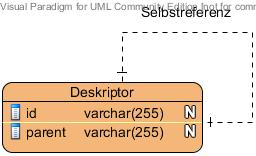
\includegraphics[scale=1]{../Bilder/selfref.jpg}
		}
		\caption{Skizze: Selbstreferenz}
		\label{fig:selfref}
	\end{figure}
	
	Die Abbildung zeigt ein Entity Relationship Diagramm als Skizze. Die 
	Zeichenlimitierung an der Zeichenkette kann hier ignoriert werden. Der Datentyp 	
	varchar kann verallgemeinert als Zeichenkette interpretiert werden. Die
	Elemente existieren nur in dieser Form aufgrund der Natur des Diagramms.
	Der wichtige Aspekt ist die Selbstreferenz. Über den Fremdschlüssel
	\emph{parent} wird ein Objekt des gleichen Typs referenziert. Dadurch kann
	ein Baum von beliebiger Tiefe erstellt werden. Ein Vater kann 
	auch beliebig viele Kinder haben, während ein Kind nur einen Vater besitzen
	kann. \\
	
	Im Folgenden soll die Anwendung dieses Modells auf die in Abschnitt
	\ref{sec:social} besprochenen Social Media Formate angewandt werden. 
	Es wird gezeigt, wie es	konzeptionell angewandt werden kann.
	
	\paragraph{Chat}\mbox{} \\
	
	Die Beziehungen in Chats sind vermutlich am Einfachsten zu beschreiben, da
	kaum welche existieren. \autoref{fig:chat_rel} zeigt ein Konzept, wie
	Beziehungen von Chats darstelltet werden können.

	\begin{figure}[H]
		\centerline{
			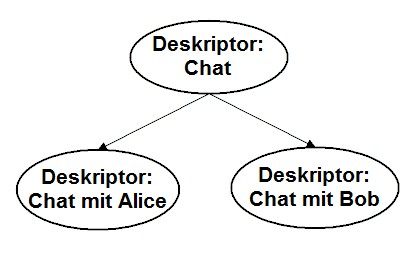
\includegraphics[scale=0.6]{../Bilder/chat_rel.jpg}
		}
		\caption{Beziehungen von Deskriptoren für Chats}
		\label{fig:chat_rel}
	\end{figure}
	
	Hier existiert genau eine Vater-Kind Beziehung. Dabei ist die
	Wurzel des Baumes nur ein Anker, der andere Deskriptoren zusammenfasst.
	Geht man nach \autoref{fig:chat_rel} so ist es möglich, alle Chats
	zu finden, indem man alle Kinder des Deskriptor Chats findet. Das
	Vaterelement soll hierbei keine Informationen oder Kontextpunkte
	beschreiben. Es dient lediglich der Zuordnung. Der Kontext kann somit als
	leer angesehen werden. Alle Kindelemente des Deskriptor Chats hingegen
	beschreiben genau einen Chat. Die zugehörigen Kontextpunkte sind somit die
	Einträge in dem Chat. Die Beziehung zwischen Deskriptoren wird hier 
	ausschließlich für die Zuordnung zu einer Obergruppe genutzt. 
		
	\paragraph{Forum und Dateisysteme}\mbox{} \\
	
	Forum und Dateisysteme gleichen sich in ihrer baumartigen Struktur. Sie können
	daher ein ähnliches Modell verwenden. Zum einen gibt es die Einordnung
	in eine Ebene, wie in ein Unterforum oder Verzeichnis. Auf der anderen
	Seite gibt es die Elemente, welche die eigentlichen Daten enthalten. \\
	
	\autoref{fig:forum_rel} zeigt ein Konzept für Beziehungen, welches die
	Einordnung von Unterforen und Threads in ein Forum darstellt.
	
	\begin{figure}[H]
		\centerline{
			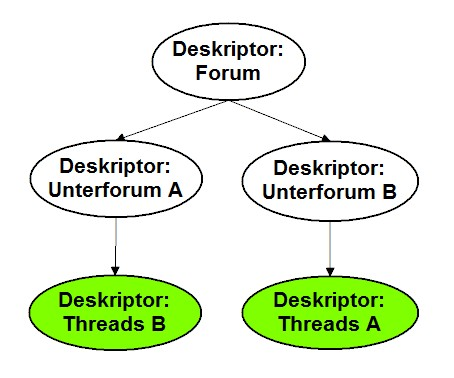
\includegraphics[scale=0.49]{../Bilder/forum_rel.jpg}
		}
		\caption{Beziehungen von Deskriptoren eines Forum}
		\label{fig:forum_rel}
	\end{figure}
	
	Abgebildet ist die Baumstruktur. Es wird an einer Wurzel begonnen und
	die Beziehungen zeigen auf, welche Unterforen von da an existieren. Die
	Deskriptoren können, wie beim Chat Deskriptor, leer sein und nur zur
	Darstellung der Beziehung verwendet werden. Zumindest Blätter müssen
	allerdings eine Menge an Kontextpunkten beschreiben. Per Konzept ist ein Thread 
	eine Menge von Kontextpunkten, wobei jeder Punkt genau einem Post entspricht.
	Demzufolge können leere Deskriptoren als reine Unterforen angesehen werden.
	Nicht leere Deskriptoren hingegen schreiben immer Threads. Ein nicht
	leerer Deskriptor mit einer Beziehung beschreibt Threads und Unterforen. \\
	
	\begin{figure}[H]
		\centerline{
			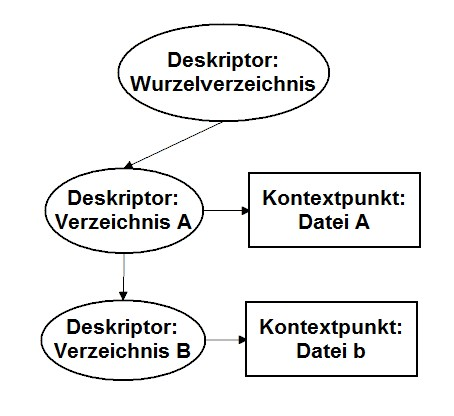
\includegraphics[scale=0.8]{../Bilder/file_rel.jpg}
		}
		\caption{Beziehungen von Deskriptoren in einem Dateisystem}
		\label{fig:file_rel}
	\end{figure}	
	
	\autoref{fig:file_rel} zeigt die Beziehungen für Verzeichnisse und Dateien.
	Die Struktur von diesen ist gleich der eines Forums. 
	Der konzeptionelle Unterschied zwischen Dateisystem und Forum ist, 
	dass ein Kontextpunkt immer genau eine Datei beschreibt. Im Forum hingegen
	beschreibt ein Thread eine Reihe von Kontextpunkten.\\
	
	Man beachte, dass es sich hierbei um ein Konzept handelt.
	Implementierungen können anders aussehen. Zum Beispiel ist es möglich und
	eventuell auch sinnvoll, dass eine Datei eine Information an einen Kontextpunkt
	ist. Somit könnte ein Kontextpunkt mehrere Dateien enthalten. Das Prinzip des
	Deskriptors ist abstrakt genug, um dem Entwickler Freiheit für seine
	Implementieren zu bieten.
	
	\subsubsection{Ein Schema für Deskriptoren}
	
	Wie bereist erwähnt gibt es in Java, der Programmiersprache in welcher die 
	zu entwickelnde Softwarekomponente geschrieben werden soll, keine vorgefertigte
	Datenstruktur für Bäume. Von daher muss eine Klasse erstellt werden, welche
	dieses ermöglicht. Im folgenden ist beschrieben, welche Aufgaben sie erfüllen
	soll.
	
	\begin{itemize}
		\item \textbf{Speichern und laden der Deskriptoren:} Das Schema soll die
		 Deskriptoren an der Wissensbasis speichern und aus dieser laden können.
		 Dies soll sowohl für alle gehen als auch für einen bestimmten
		 Identifikator.
		\item \textbf{Vater-Kind Beziehung:} Das Schema stellt die eigentlichen
		Vater-Kind Beziehungen dar. Daher ermöglicht es einem Deskriptor, Kinder
		hinzuzufügen, sowie einen Vater zu setzen. Wird ein neuer Vater gesetzt,
		wird der alte überschrieben. Auch muss sichergestellt werden, dass
		es zu keiner Schleife bei den Bezeichnungen kommt, damit immer ein Baum
		mit einer Wurzel und Blättern existiert.
	\end{itemize}
	
	\subsubsection{Extraktion von Daten}
	\label{sec:extraction}
	
	Deskriptoren existieren um Datenbereiche zu beschreiben. Als solches 
	muss die Möglichkeit bestehen, Kontextpunkte anhand des Kontext eines Deskriptors
	zu extrahieren. Dabei sollen die folgenden Möglichkeiten bestehen:
	
	\begin{itemize}
		\item \textbf{Extraktion des Kontext des Deskriptors:} Nur die Kontextpunkte
		zum Kontext des aktuellen Deskriptors werden extrahiert.
		\item \textbf{Extraktion des Unterbaumes:} Die Kontextpunkte des aktuellen
		 Deskriptor, sowie alle Kontextpunkte seiner Kinder werden extrahiert
		\item \textbf{Extraktion des gesamten Baumes:} Die gesamten Kontextpunkte
		des Baumes werden extrahiert. Das heißt, es wird zuerst die Wurzel des
		Baumes gesucht und dann der Unterbaum, inklusive der Wurzel selbst,
		extrahiert.
	\end{itemize}
	
	\subsection{Synchronisation}
	
	In diesem Abschnitt wird der Algorithmus zur Synchronisation der Daten
	konzipiert. Dazu wird der Algorithmus der SyncKB von des Shark Framework 
	mit dem im letzten Abschnitt beschriebenen Deskriptor erweitert.
	
	\subsubsection{Mängel der aktuellen SyncKB}
	
	Bevor ein Algorithmus entworfen wird, sollen die Mängel der aktuellen 
	Synchronisation besprochen werden. \autoref{fig:sync_now} zeigt nochmal eine
	Skizze des Algorithmus des SyncKP aus Abschnitt \ref{sec:SyncKB}. Für 
	eine Erklärung des sequenziellen Ablauf siehe \autoref{fig:SyncSeq}. \\
	
	In der aktuellen Form zeigt der Algorithmus der SyncKB zwei gravierende Mängel
	auf.
	
	\begin{enumerate}
		\item \textbf{Synchronisation mit allen Peers:} Der Algorithmus nimmt alle
		Peers der Wissensbasis und synchronisiert mit diesen. Für die
		Fallbeispiele dieser Arbeit soll aber nur mit bestimmten Peers eine
		Synchronisation stattfinden. So wären dies beispielsweise in einem Chat die
		Teilnehmer, in einem Forum alle Mitglieder dieses. Diese Menge ist
		nicht zwangsweise gleich mit allen Peers in der Wissensbasis.
		\item \textbf{Synchronisation aller Kontextpunkte:} Ebenfalls
		synchronisiert der Algorithmus alle Kontextpunkte einer Wissensbasis. 
		Dem Namen dieser Arbeit nach ist allerdings eine partiellen Synchronisation
		erwünscht.		
	\end{enumerate}
	
	\begin{figure}[H]
		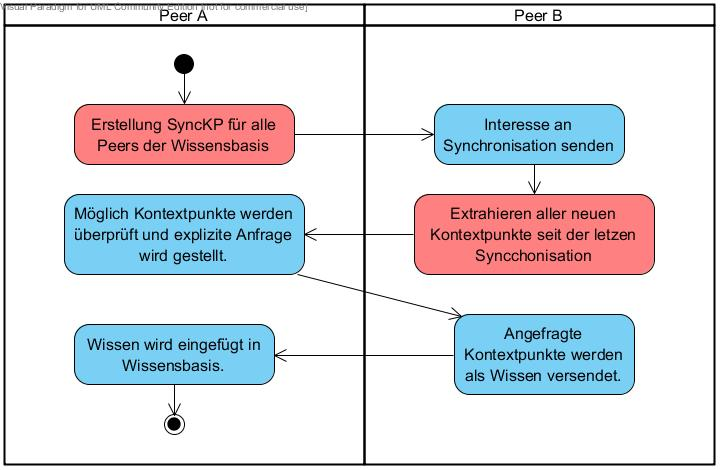
\includegraphics[width=\linewidth]{../Bilder/sync_flaws.jpg}
		\caption{Skizze: Synchronisation Algorithmus der aktuellen SyncKB}
		\label{fig:sync_now}
	\end{figure}
	
	\subsubsection{Abstraktion von der SyncKB}
	\label{sec:sync_abstract}
	
	Aufgrund der im letzten Abschnitt beschriebenen Mängel soll eine Abstraktion der
	SyncKB vorgenommen werden. Genauer soll die Klasse SyncKP abstrahiert werden.
	Wenn hier von einer Abstraktion gesprochen wird, dann ist von einer Abstraktion 
	im Sinne der objektorientierten Programmierung die Rede.
	Die Klasse SyncKP soll in
	eine abstrakte Klasse AbstractSyncKP umgewandelt werden. Der Entwickler, der
	von dieser erbt, ist dann verpflichtet die abstrakten Methoden 
	zu implementieren. Ziel der Methoden ist das erreichen folgender Aktionen:
	
	\begin{itemize}
		\item \textbf{Entscheidung ob ein Interesse besteht:} Es sollte im 
		Ermessen des Entwicklers liegen, ob ein Interesse
		für eine Knowledge Port interessant ist oder nicht. Je nach Fall kann
		es vorkommen, dass bestimmte Dimensionen des gesendeten Interesses überprüft
		werden müssen oder nicht. Dem Entwickler soll hier Freiheit gegeben werden,
		dies selbst zu entscheiden.
		\item \textbf{Finden des Identifikator:} Die bestehende Implementation der
		SyncKB benötigt einen Identifikator an dem es seine Metadaten speichern
		kann. Dieser Identifikator ist nicht gleich mit dem Identifikator eines
		Deskriptor. Es handelt sich um ein tatsächliches Tag an dem Properties
		gespeichert werden können. Im künstlichen Interesse der aktuellen SyncKB
		ist dies ein Tag in der Topic Dimension, dass schlicht dem halten von
		Metadaten dient.
		\item \textbf{Zusammenstellen des Angebotes:} Wie in Abschnitt
		\ref{sec:extraction} erläutert, gibt es mehrere Möglichkeiten, Wissen
		anhand eines Deskriptors zu extrahieren. Daher ist es sinnvoll, dem
		Entwickler zu überlassen, wie genau das Wissen aus der Wissensbasis
		extrahiert wird. 
	\end{itemize} 	
	
	\subsubsection{Eliminierung des Piggyback Algorithmus}
	\label{sec:piggyback}
	
	Wie in \autoref{fig:SyncSeq} aus Abschnitt \ref{sec:SyncKB} zu sehen ist,
	benutzt die aktuelle SyncKB Implementierung einen Piggyback Algorithmus.
	Sinn dieses ist es, den Datenaustausch möglichst gering zu halten. Erste Tests
	mit einer abstrakten Version der SyncKP Klasse haben aber gezeigt, dass
	dies zu einer langen Laufzeit des Algorithmus führen kann, selbst wenn die
	Daten nur lokal ausgetauscht werden. Dieser führte sogar in vielen Fällen
	zu einer SocketException mit der Fehlerbeschreibung \emph{Software caused
	connection abort: socket write error}. Dadurch wurde der Algorithmus abgebrochen
	ohne das Wissen gesendet wurde und die Synchronisation schlug fehl. 
	Nach einem Post auf stackoverflow \cite{sockError} kann dies auftreten, wenn 
	der Empfänger nie den Empfang der Daten bestätigt. Da der Fehler nach der
	Vereinfachung verschwand, ist anzunehmen, dass die Komplexität des Algorithmus
	gekoppelt mit weiteren Algorithmen zur partiellen Synchronisation die Ursache
	hierfür ist. Aus diesem Grund wurde der Piggyback Algorithmus entferne.\\
	
	In \autoref{fig:sync_flow_concept} ist der, verglichen mit \autoref{fig:SyncSeq},
	vereinfachte Algorithmus skizziert.
	
	\begin{figure}[H]
		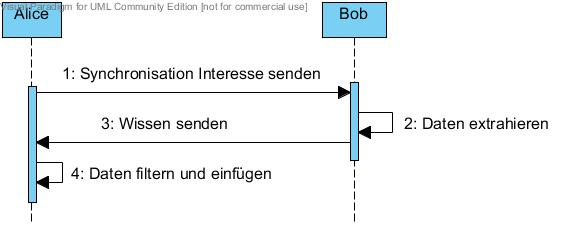
\includegraphics[width=\linewidth]{../Bilder/sync_flow_concept.jpg}
		\caption{Vereinfachter Algorithmus zur Synchronisation}
		\label{fig:sync_flow_concept}
	\end{figure}
	
	Der Ablauf wurde auf folgende Schritte vereinfacht:
	
	\begin{enumerate}
		\item \textbf{Interesse senden:} Wie im alten Algorithmus versendet Alice
		zuerst ein Interesse an einer Synchronisation.
		\item \textbf{Daten extrahieren:} Bob erreicht dieses Interesse. Bob
		wird nun explizit das Wissen extrahieren. Er macht keinen Vorschlag an
		möglichen Kontextpunkten sondern sendet das Wissen direkt zu. Auch
		hier werden wieder alle Kontextpunkte und zugehörige Themen und Peers
		gesendet, die nach dem letzten Treffen mit dem Kommunikationspartner
		aktualisiert wurden.
		\item \textbf{Wissen senden:} Das gesamte Wissen wird nun an Alice gesendet.
		Alice prüft nicht mehr, welche Kontextpunkte sie benötigt und stellt auch
		keine Anfrage nach bestimmten Kontextpunkten mehr. Sie erhält alles, was
		Bob extrahiert hat.
		\item \textbf{Daten filtern und einfügen:} Alice überprüft nun, welche
		Kontextpunkte sie einfügen will. Dies ist identisch zu dem Algorithmus,
		der im rechten Teil von \autoref{fig:SyncFlow} skizziert und unter der
		Abbildung erklärt ist.
	\end{enumerate} 	
		
	Vorteil dieser Eliminierung ist, dass der Algorithmus leichter zu verstehen ist 
	und	der Quellcode somit leichter gewartet werden kann. Nachteil ist, dass
	potenziell eine große Menge an Wissen versendet wird, der 
	Kommunikationspartner aber nur einen geringen Teil einfügt. Dies ist aber
	dem Erzeugen eines Fehlers vorzuziehen. Besonders, da in der zu entwickelnden
	Softwarekomponente nur Teilbereiche von Wissensbasen synchronisiert werden
	sollen. Daher kann davon ausgegangen werden, dass die Datenmengen generell
	relativ klein ausfallen. Zusätzlich ist es einen Nutzer leicht verständlich zu
	machen, dass das Senden von großen Datenmengen eine gewisse Zeit beanspruchen
	kann. Dies kennt er eventuell vom Versenden von E-Mails mit großen Anhängen.
	Eine lange Laufzeit einer Sequenz von Befehlen ist eher selten verständlich für
	Nutzer.	 
	
	\subsubsection{Ein synchronisierbares Schema}
	
	Das Schema ist nicht von sich aus synchronisierbar. Grund hierfür ist, dass es
	auf einer einfachen Wissensbasis beruht. Für die Synchronisation wird aber
	eine Wissensbasis benötigt, die als SyncKB implementiert ist. Da diese,
	wie in Abschnitt \ref{sec:SyncKB} erklärt, nur ein Wrapper ist, kann hier per
	Ableitung  eine	Kindklasse erstellt werden. Diese nimmt anstatt einer normalen
	Wissensbasis nur eine SyncKB entgegen und bietet eine Methode an, die SyncKB per
	Getter vom Schema zu erhalten. Da bei der Synchronisation oft der Eigentümer
	der Wissensbasis benötigt wird soll dieser ebenfalls überprüft werden. Wenn
	dieser fehlt, soll bei der Initialisierung ein Fehler auftreten. \\
	
	Über diesen einfachen Schritt wird ein Schema erzeugt, das immer auf einer
	SyncKB beruht und dessen Wissensbasis immer einen Eigentümer hat. Die
	abgeleitete Klasse ist somit ein Vertrag zur Versicherung, dass diese
	Bedingungen erfüllt sind.
	
	\subsubsection{Ein künstliches Interesse}
	\label{sec:artificial_interest}
	
	Wie bei der ursprüngliche Implementierung der SyncKB soll auch hier ein
	künstliches Interesse genutzt werden. Der Grund hierfür ist, dass ein
	Interesse im Shark Framework keinen Platz für Metadaten bietet. \\
	
	Die Dimensionen sind nachfolgend beschrieben. \autoref{fig:artificial_context}
	zeigt eine Skizze für den Aufbau des künstlichen Interesses.
	
	\begin{itemize}
		\item \textbf{Topics:} Die Topics Dimension soll genau ein SemanticTag
		enthalten. Dieses ist ein Thema, dass keiner Beschreibung
		dient. An dem Thema sollen nur Properties gesetzt werden, die Metadaten
		entsprechen. Der Deskriptor selbst soll als XML an ihr gespeichert werden.
		Somit wird die Topics Dimension zu einer Metadaten Dimension umdefiniert.
		In dieser Dimension wird sich daher auch immer nur dieses eine Thema finden,
		welches die Metadaten hält.
		\item \textbf{Peers:}  Die Peers Dimension stellt die Person da, die das
		Interesse an einer Synchronisation versendet. Geplant ist, dass dies
		immer nur eine einzelne Person ist. Genauer der eigen Eigentümer
		des Schemas, zu dem der Deskriptor gehört.
		\item \textbf{Remote Peers:} Die Remote Peers Dimension sind die Personen,
		bei denen eine Synchronisation angefragt wird. Das heißt von diesen
		Personen wird Wissen empfangen und eventuell in die Wissensbasis eingefügt.
		Gegenüber anderen Dimension können sich in dieser mehre Elemente befinden.
		Das heißt, man kann sich mit mehreren Personen synchronisieren.
		Die aktuellsten Daten werden dabei in die Wissensbasis eingefügt.
		\item \textbf{Direction:} Die Direction Dimension gibt an, ob ein 
		Knowledge Port aktiv ist. Dies kann ähnlich einer Subscription gesehen
		werden.	Ist ein Knowledge Port abonniert, so wird dieser Daten versenden 
		und	empfangen. Dies entspricht dem Verhalten der Direction INOUT. Ist ein
		Knowledge Port nicht abonniert, wird er weder Daten senden noch sie
		empfangen. Dies entspricht dem Verhalten der Direction NOTHING.
	\end{itemize} 	
	
	Die Dimensionen Originator, Times und Locations sind für den
	Algorithmus zur	Synchronisation unerheblich und bleiben daher leer.
	
	\begin{figure}[H]
		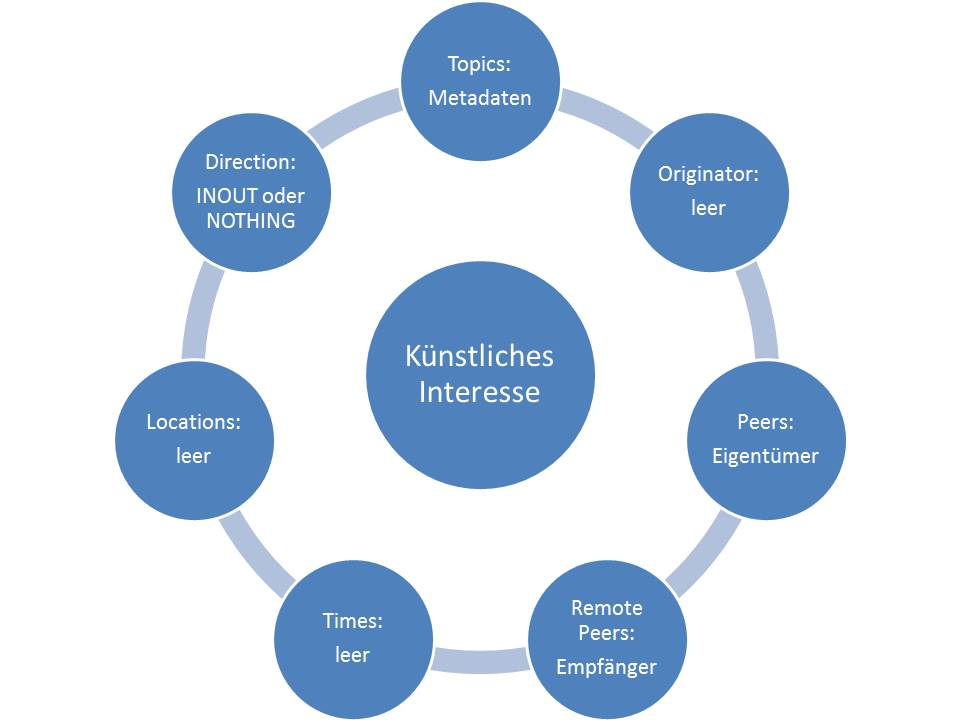
\includegraphics[width=\linewidth]{../Bilder/artificial_context.jpg}
		\caption{Skizze: Künstliches Interesse für partielle Synchronisation}
		\label{fig:artificial_context}
	\end{figure}
	
	\subsubsection{Pull und Pull Request}
	\label{sec:pull}
	
	In dieser Arbeit, sowie in der Implementierung der vorhandenen SyncKB, ist
	von Synchronisation die Rede. In der Realität ist der beschriebene 
	Algorithmus aber eher einem Pull, bekannt aus der Versionsverwaltung
	Software Git, gleichzusetzen. Dies bedeutet, dass die Synchronisation
	einseitig ist. Nur der Peer, welcher das Interesse sendet, bekommt Daten
	zugesandt. Die Wissensbasis des Peers, der die Daten sendet, ändert sich nicht.
	Das heißt, dass Peer A alle Daten, die durch einen Deskriptor beschrieben sind,
	von Peer B erhalten wird. Peer B hingegen wird eventuell nicht alle Daten von
	Peer A besitzen, die durch den Deskriptor beschrieben sind.
	
	Zu diesem Zweck soll in zwei Aktionen unterschieden werden: 
	Pull und Pull Request.
	
	\begin{itemize}
		\item \textbf{Pull:} Ein Pull entspricht dem in
		\autoref{fig:sync_flow_concept} skizzierten Algorithmus. Hier werden
		Daten von einem entfernten Peer geholt und in die eigene Wissensbasis
		eingefügt. Der Kommunikationspartner erhält keine Daten und somit ändert
		sich sein Datenbestand nicht.
		\item \textbf{Pull Request:} Ein Pull Request ist nichts anderes als eine
		andere Person um ein Pull zu bitten. Dies hat zur Folge, dass diese
		Person alle Daten vom Antragsteller bekommt. Der eigene Datenbestand 
		ändert sich hier nicht. Nur die Wissensbasis der Person, welche die
		Anfrage erhält, wird aktualisiert.	
	\end{itemize} 
	
	Eine vollständige Synchronisation wäre somit ein Pull gefolgt von einem
	Pull Request. Im Rahmen dieses Konzeptes soll dies nicht implementiert werden.
	Grund hierfür ist, dass zum	Zeitpunkt dieser Arbeit keine Möglichkeit besteht 
	zu erkennen, wann die Kommunikation eines Knowledge Port beendet ist. 
	Es ist nicht klar, wann ein Pull beendet ist und der Pull Request gestartet 
	werden kann. Dieser Aspekt wird somit als Mangel des zugrundeliegenden
	Algorithmus gesehen und aus zeitlichen Gründen vernachlässigt.
	
	\subsubsection{Eine weitere Abstraktionsebene}	
	
	Neben der Abstraktion des SyncKP ist eine weitere Abstraktionsebene geplant.
	Das künstliche Interesse sowie die Nutzung der Deskriptoren soll in
	dieser Ebene geschehen. \autoref{fig:ebene} zeigt eine Skizze der
	Abstraktionsebenen,	die verwendet werden sollen.
	
	\begin{figure}[H]
		\centerline{
			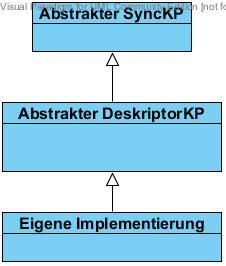
\includegraphics[scale=0.6]{../Bilder/ebene.jpg}
		}
		\caption{Skizze: Abstraktionsebenen}
		\label{fig:ebene}
	\end{figure}	
	
	In der ersten Ebene liegt der eigentliche Algorithmus zur Synchronisation.
	In der zweiten Ebene wird dieser so angepasst, dass er auf Grundlage
	eines Deskriptors geschieht. Die letzte Ebene wird vom Entwickler selbst
	implementiert. Sie enthält alle Funktionen, die vom Anwendungsfall abhängen. \\
	
	Geplant ist, dass die Deskriptor Ebene folgende Funktionen anbietet bzw.
	übernimmt:
		\begin{itemize}
		\item \textbf{Senden eines Deskriptors:} Sollte der Deskriptor geändert
		werden, kann die Änderung an die Kommunikationspartner
		verteilt werden. Die anderen Peers überschreiben dabei den Deskriptor
		in ihrem Schema mit dem neuen Inhalt.
		\item \textbf{Senden von geänderten Adressaten:} Die Personen, mit 
		denen eine Synchronisation erfolgen soll, können sich ändern. Die
		Deskriptor Ebene bietet an, Adressaten hinzuzufügen und zu entfernen.
		Wie mit dieser Änderung umzugehen ist, muss allerdings jeder Entwickler
		in der letzten Ebene selbst bestimmen.
		\item \textbf{Finden des Identifikators:} Es wird das künstliche Interesse
		genutzt. Das Thema in der Topic Dimension, das die Metadaten hält, soll
		dabei als Identifikator dienen.
		\item \textbf{Interesse bekunden:} Die Deskriptor Ebene übernimmt das
		Prüfen des Interesses. Sie entscheidet, ob eine Kommunikation stattfindet.
		Dies ist der Fall, wenn die Deskriptoren die Gleichheit aufweisen, also
		ihr Identifikator gleich ist.
		\item \textbf{Subskription:}  Je nach Status einer Subskription wird der
		Knowledge Port Daten versenden und empfangen oder inaktiv sein.		
	\end{itemize} 
	
	Für die eigene Implementierung durch den Entwickler bleiben somit folgende
	Tätigkeiten übrig:
	
	\begin{itemize}
		\item \textbf{Senden eines Deskriptors:} Der Entwickler bestimmt, wie
		genau Daten extrahiert werden. Das einspricht dem Zusammenstellen des
		Angebotes der Abstraktion des SyncKP (vergleiche Abschnitt
		\ref{sec:sync_abstract}).
		\item \textbf{Auf geänderten Adressaten reagieren:} Es liegt in der
		Zuständigkeit eines jeden Entwicklers wie auf Änderungen der Adressaten
		reagiert wird. Eine entsprechende Vorgehensweise muss implementiert 
		werden.
	\end{itemize} 
	
	\subsection{Lernen von Deskriptoren}
	
	Es wurde ein Konzept zum Aufbau von Deskriptoren, sowie einer Synchronisation
	auf deren Grundlage erstellt. Da Deskriptoren aber nicht immer vordefiniert
	vorhanden sein müssen, soll auch ein Konzept zum Lernen dieser erstellt werden. 
	Dabei soll sich einer sehr einfachen Methode bedient werden. \\
	
	Um anderen Kommunikationspartnern ein Deskriptor beizubringen wird er über
	einen, von den anderen Algorithmen unabhängigen, Knowledge Port versandt.
	Dabei wird nicht der Deskriptor selbst übertragen, sondern sein gesamter Baum.
	Andere Peers fügen diesen Baum dann in ihr Schema ein. Dabei werden alle
	existierenden Deskriptoren mit dem gleichen Identifikator überschrieben. 
	Das kann natürlich unerwünscht sein, weshalb die entsprechende Klasse
	so gebaut sein soll, dass über Ableitung eine Anpassung des Verhaltens
	möglich ist.
	
	\newpage
	\section{Implementierung}
	
	In diesem Kapitel wird die Implementierung besprochen. Es wird gezeigt, wie
	das Konzept in Java Quellcode implementiert wurde und welche Techniken dazu
	verwendet wurden. Des Weiteren wird besprochen, wie entworfene Klassen 
	genutzt werden können.
	
	\subsection{Deskriptor und Schema}
	
	Im folgenden Abschnitt wird auf die Implementierung des Deskriptors und Schemas
	eingegangen. Es wird erklärt, welche Eigenschaften sie haben und wie sie benutzt
	werden können.
	
	\subsubsection{Die Klassen ContextSpaceDescriptor und DescriptorSchema}
	
	Deskriptor und Schema werden in die zwei Klassen ContextSpaceDescriptor
	und DescriptorSchema aufgeteilt. Die Klasse ContextSpaceDescriptor ist dabei
	eine reine Beschreibung eines Datenbereiches. Die Klasse DescriptorSchema
	organisiert die Deskriptoren in einer Baumstruktur und ermöglicht das
	Speichern und Laden dieser von einer Wissensbasis. \autoref{fig:impl_schema}
	zeigt das Klassendiagramm beider.
	
	\begin{figure}[H]
		\centerline{
			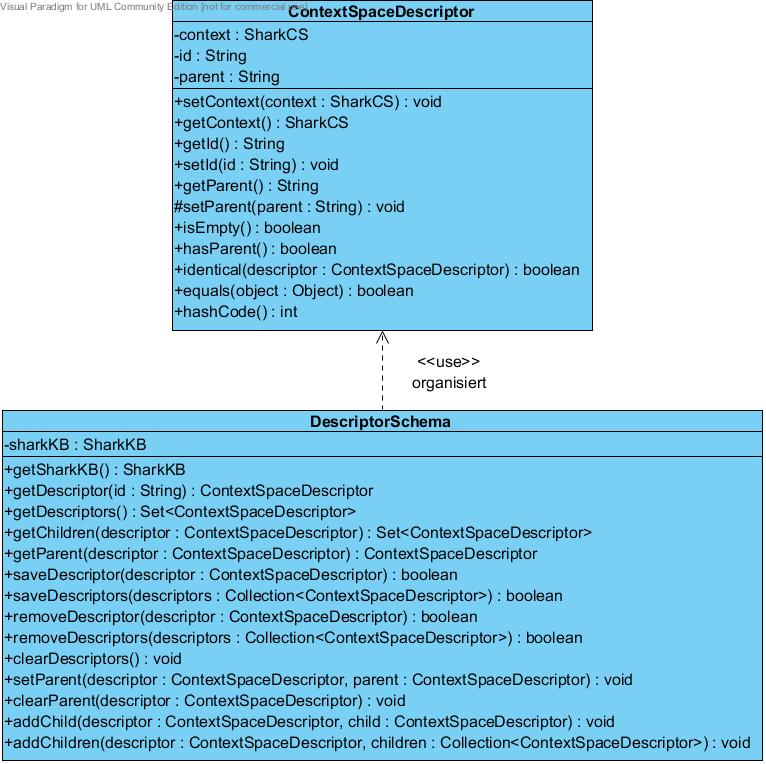
\includegraphics[scale=0.53]{../Bilder/impl_schema.jpg}
		}
		\caption{Klassendiagramm: Deskriptor und Schema}
		\label{fig:impl_schema}
	\end{figure}	
	
	Konstruktoren und private Methoden wurden hier vernachlässigt. Eine
	explizite Beschreibung aller Klassen kann in der JavaDoc Dokumentation gefunden
	werden (siehe \autoref{sec:CD}). \\
	
	Im folgenden wird auf die Verwendung dieser Klassen eingegangen.
		
	\paragraph{Deskriptor}\mbox{} \\
	
	Die Klasse ContextSpaceDescriptor hat die aus Abschnitt \ref{sec:desk} 
	beschriebenen drei Parameter Kontext (context), Vater (parent) und
	Identifikator (id). Für diese Methoden gibt es jeweils Setter und Getter
	Methoden. Zu beachten dabei ist, dass der Setter für den Vater auf die
	Sichtbarkeit protected gesetzt ist. Der Entwickler soll die	Vater-Kind
	Beziehungen über das Schema konfigurieren, welche Fehlerprüfungen durchführt,
	nicht über die Klasse ContextSpaceDescriptor selbst. Das der Getter für
	parent die Sichtbarkeit public besitzt dient nur zu Debugging und Logging
	Zwecken.\\
	
	Des Weiteren gibt es eine Reihe von Methoden, welche folgende Eigenschaften
	prüfen:
	
	\begin{itemize}
		\item \textbf{Leere:} Die isEmpty Methode prüft, ob ein Deskriptor
		leer ist. Ein Deskriptor ist leer, wenn der Parameter context null ist.
		\item \textbf{Zwei Deskriptoren sind gleich:} Die von Object überschriebene
		equals Methode pürft ob zwei Deskriptoren gleich sind. Ein Deskriptor
		gleicht einem anderen, wenn die Parameter id gleich sind. Mit dieser
		Prüfung	auf Gleichheit werden Features des Collection Framesworks 
		von Java genutzt. Die contains Methode zum Beispiel gibt so wieder, ob
		in einer Collection bereits ein Deskriptor mit dem gleichen Identifikator
		existiert. Zusätzlich ist auch die hashSet Methode überschrieben. Das
		ausschlaggebende Element ist auch hier der Parameter id. Demzufolge
		ist auch der Hash zweier Deskriptoren gleich, wenn ihr Identifikator 
		gleich ist.
		\item \textbf{Zwei Deskriptoren sind identisch:} Die identical Methode
		prüft, ob ein Deskriptor identisch zu einem anderen Deskriptor ist. Dies
		ist der Fall, wenn die Parameter id und parent die Gleicheit aufweisen,
		sowie die context Parameter identisch sind nach den Regeln des Shark
		Frameworks. Somit können Deskriptoren auf Unterschiede geprüft werden,
		obwohl sie den gleichen Identifikator besitzen.
	\end{itemize}
	
	\paragraph{Schema}\mbox{} \\
	
	Die Klasse DescriptorSchema ermöglicht sowohl das Speichern, wie auch das
	Laden von Deskriptoren aus der Wissensbasis. Des Weiteren können die
	Beziehungen	zwischen Deskriptoren konfiguriert werden.
	Nach außen ist sie die Klasse, welche die Beziehungen enthält, auch wenn die
	Schlüssel intern an der Klasse ContextSpaceDescriptor beschrieben sind. Sie kann
	ähnlich einem Datenbankmanagementsystem gesehen werden. \\
	
	Ein Schema basiert immer auf einer Wissensbasis, aus der die Daten geladen und
	gespeichert werden. Des weiteren besitzt sie folgende Features:
	
	\newpage
	\begin{itemize}
		\item \textbf{Speichern und Laden von Deskriptoren:} Deskriptoren können
		an der Wissensbasis, die das Schema verwendet, gespeichert und
		geladen werden. Hierzu enthält die Klasse die Methoden getDescriptor,
		getDescriptors, saveDescriptor, saveDescriptors, removeDescriptor und
		saveDescriptors. Das Löschen des gesamten Schemas ist mittels 
		clearDescriptors möglich. Deskriptoren werden immer in einem Set gehalten,
		das heißt alle Elemente der Liste sind unterschiedlich. Unterschiedlich
		bezieht sich hierbei auf die Gleichheit, das heißt sie besitzen alle
		unterschiedliche Identifikatoren. Das Speichern eines Deskriptors mit dem
		gleichen Identifikator wie ein bereits existierender Deskriptor,
		kommt einem Überschreiben gleich.
		\item \textbf{Konfigurieren von Vater-Kind Beziehungen:} Über die Methoden 
		addChild, addChildren, setParent können Vater-Kind Beziehungen aufgebaut
		werden. Zu beachten ist, dass ein Deskriptor immer nur einen Vater
		haben kann. Wird ein Neuer gesetzt, so wird der Alte überschrieben. Das
		hinzufügen eines Kindes zu einem Deskriptor ist gleich dem Setzen eines 
		Vaters (Parameter: descriptor) für den Parameter child. Existiert ein
		Deskriptor nicht im Schema oder würde das Hinzufügen zu einer
		Schleife führen, also die Baumstatur verletzen, erzeugt dies einen
		Fehler.	Ein Vater kann über die clearParent Methode gelöscht werden. Über
		die getChildren	und getParent können Vater und Kinder eines Deskriptors
		erhalten werden.
	\end{itemize}
	
	Neben den dargestellten Methoden existieren weitere statische Methoden um Eltern
	und Kinder in einer java.util.Collection zu finden. Auch existieren Methoden die
	Aussagen geben, ob sich im Schema bereits ein gleicher oder identischer
	Deskriptor befindet. Weiteres kann in der JavaDoc Dokumentation 
	(siehe \autoref{sec:CD}) nachgeschlagen werden.
	
	\subsubsection{Serialisierung des Schemas}
	
	Wie in Abschnitt \ref{sec:konz_serialisierung} erklärt, soll XML unter
	Zuhilfenahme des im Java Development Kit enthaltenen JAXB zum Serialisieren
	des Schemas verwendet werden. Hierzu ist die Klasse ContextSpaceDescriptor
	mit entspreche Annotations ausgestattet. Für den Parameter context wurde
	ein entsprechender XmlAdapter (siehe \cite{XmlAdapter}) geschrieben, der
	die Serialisierung einer SharkCS Klasse unter Zuhilfenahme der im Shark
	Framework existierenden Klasse XMLSerializer für JAXB ermöglicht. \\
	
	Aufgrund der Annotations wurde auch drauf verzichtet, ein Interface zur Klasse
	ContextSpaceDescriptor zu erstellen oder sie abstrakt zu gestalten. Sie wurde
	als normales Java Objekt entworfen, das einfach wie eine Java-Bean genutzt
	werden kann. \\
	
	In der JAXB 2.2 Specification, Section 4.2 JAXB Context \cite{JAXB} steht
	folgendes beschrieben: 
	
	\emph{
		\begin{quote} 
			"To avoid the overhead involved in creating a JAXBContext instance,
			a JAXB application is encouraged to reuse a JAXBContext instance."
		\end{quote}
	} 

	\newpage
	Aus diesem Grund wurde das Factory Pattern für die Erstellung eines
	JAXBContext	benutzt. \autoref{fig:factory} skizziert dieses.
	
	\begin{figure}[H]
		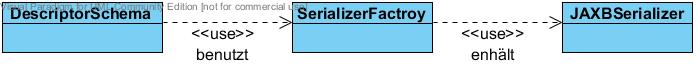
\includegraphics[width=\linewidth]{../Bilder/factory.jpg}
		\caption{Skizze: Factroy Pattern für JAXB Serialisierung}
		\label{fig:factory}
	\end{figure}	
	
	Der JAXBContext ist in der Klasse JAXBSerializer enthalten. Für jede Instanz
	dieser Klasse wird ein neuer JAXBContext angelegt. Um dies zu verhindern wird
	die Factory Klasse SerializerFactroy benutzt. Diese folgt dem Singleton Pattern
	und enthält genau einen JAXBSerializer der für Deskriptoren konfiguriert ist. 
	Das Schema kann diesen über eine Methode abrufen. Sollten weitere Klassen
	einen JAXBSerializer für Deskriptoren benötigen, kann die Instanz 
	über SerializerFactroy wiederverwendet werden. Somit wird auch der JAXBContext
	wiederverwendet und Overhead vermieden.
	
	\subsubsection{Algorithmen für die Extraktion von Daten}
	
	Wie in Abschnitt \ref{sec:extraction} beschrieben gibt es drei Arten der
	Extraktion von Daten. Als Implementierung wurde hierzu die Klasse
	DescriptorAlgebra geschrieben. Diese hält nur statische Methoden, welche die
	entsprechenden drei Extraktionen ausführen. 
	
	\paragraph{Extraktion des Kontextes eines Deskriptor}\mbox{} \\
	
	Für den Algorithmus der Extraktion des Kontextes eines Deskriptors wird
	die vom Shark Framework bereitgestellte Klasse SharkCSAlgebra genutzt.
	Die Kontextpunkte werden anhand des Kontextes des Deskriptors und einer
	übergebenen Wissensbasis extrahiert.
	
	\paragraph{Extraktion des Unterbaumes}\mbox{} \\
	
	Der Algorithmus für die Extraktion eines Unterbaumes ist im linken Teil von
	\autoref{fig:extraction} dargestellt. Zuerst wird das Wissen des aktuellen
	Knoten wie bei der Extraktion des Kontext eines Deskriptors extrahiert.
	Danach werden die Kinder des aktuellen Deskriptors ermittelt. Existieren
	Kinder, kommt es zu einem rekursiven Aufruf. Dieser wird bis zu den Blättern
	des Baumes laufen und das Wissen eines Blattes zurückliefern. Danach wird
	im Vaterknoten das Wissen des Kindes mit dem Wissen des Vaters vereint (nicht 
	abgebildet) und das Wissen des nächsten Kindes wird extrahiert. Dies geschieht
	bis zum Anfangsknoten. Schließlich wird das Wissen dieses mit dem Wissen der
	Kinder vereint. Somit werde alle Kontextpunkte des aktuellen
	Deskriptor,	sowie aller seiner Kinder, gefunden. Dabei wird auch auf Gleichheit
	dieser geprüft, damit kein Kontextpunkt im Wissen doppelt vorkommt. Die
	Gleichheitsprüfung erfolgt über die von Object geerbt equals Methode einer jeden
	Java Klasse.
	
	\newpage
	\paragraph{Extraktion des gesamten Baumes:}\mbox{} \\
	
	Bei der Extraktion des gesamten Baumes wird zuerst die Wurzel gesucht. Das heißt,
	es wird solange die Vaterkette entlang gegangen, bis ein Knoten in dieser keinen 		Vater mehr besitzt. Im Anschluss erfolgt eine Extraktion des Unterbaumes. Da
	hier von der Wurzel ausgegangen wird, entspricht eine Extraktion des Unterbaumes
	einer Extraktion des gesamten Baumes. Skizziert ist das im linken Teil von
	\autoref{fig:extraction}. \\
	
	Die Suche nach der Wurzel in diesem Algorithmus ist auch der Grund, warum
	im Schema streng eine Baumstruktur genutzt wird mit je einem Vater und keine
	Schleifen auftauchen dürfen. Andernfalls könnte keine Wurzel gefunden werden.
	
	\begin{figure}[H]
		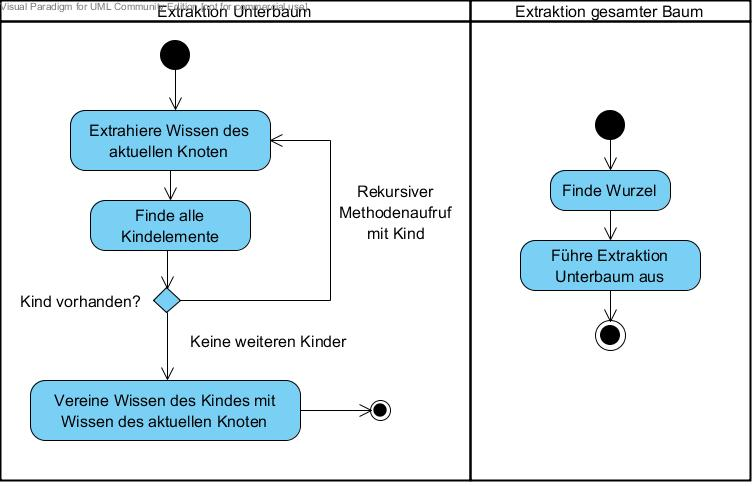
\includegraphics[width=\linewidth]{../Bilder/extraction.jpg}
		\caption{Skizze: Algorithmus Extraktion}
		\label{fig:extraction}
	\end{figure}	
	
	\subsection{Synchronisation von durch Deskriptoren beschriebenen Datenbereichen}	
	
	Im folgenden Abschnitt werden die Techniken und Algorithmen besprochen, die
	zur Synchronisation von durch Deskriptoren beschriebenen Datenbereichen genutzt
	werden.
	
	\subsubsection{Die abstrakte Klasse AbstractSyncKP}
	
	Die Klasse SyncKP wurde abstrahiert, um sie allgemeiner einsetzen zu können.
	Die erwähnte Eliminierung des Piggyback Algorithmus aus Abschnitt
	\ref{sec:piggyback} ist hierbei die größte Änderungen. Dadurch fallen die 
	Phasen Angebot und Anfrage weg. Außerdem hat die neue Klasse
	AbstractSyncKP einige neue Methoden. Die Wichtigsten sind im Klassendiagramm
	in \autoref{fig:AbstractSyncKP} dargestellt.
	
	\begin{figure}[H]
		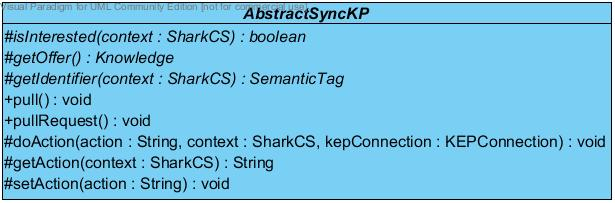
\includegraphics[width=\linewidth]{../Bilder/AbstractSyncKP.jpg}
		\caption{Klassendiagramm: AbstractSyncKP}
		\label{fig:AbstractSyncKP}
	\end{figure}	
	
	Die abstrakten Methoden besitzen die Sichtbarkeit protected. Sie 
	müssen von jeder Kindklasse implementiert werden. In
	\autoref{fig:abstract_algorithm} ist hervorgehoben, wo
	die Methoden während der Synchronisation Verwendung finden werden. 
	
	\begin{figure}[H]
		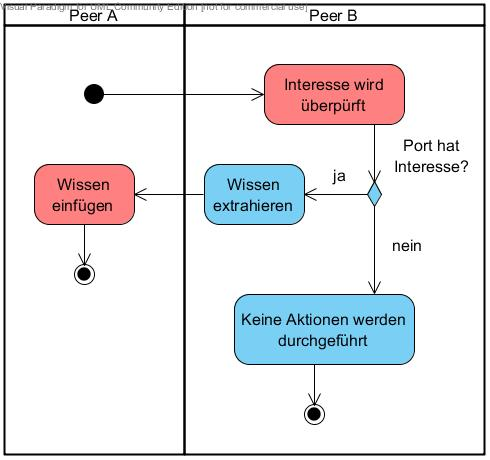
\includegraphics[width=\linewidth]{../Bilder/abstract_algorithm.jpg}
		\caption{Ablauf einer Synchronisation}
		\label{fig:abstract_algorithm}
	\end{figure}	
		
	\newpage
	\begin{itemize}
		\item \textbf{Interesse bekunden:} Zuerst muss herausgefunden werden,
		ob das erhaltene Interesse überhaupt relevant ist. Die Implementierung
		hierzu ist jedem Entwickler selbst überlassen. So kann beispielsweise
		gegen eine Blacklist geprüft werden, da man mit bestimmten Personen
		gar nicht kommunizieren möchte. Natürlich muss hier auch implementiert 
		werden, ob das erhaltene Interesse überhaupt ein Interesse zur
		Synchronisation ist. Nur wenn diese Methode true zurückliefert, werden
		weitere Aktionen durchgeführt.
		\item \textbf{Wissen extrahieren:} Die Extraktion des benötigten Wissens 
		kann sich je nach Einzelfall unterscheiden. Dem Entwickler wird hier die
		Freiheit gelassen, wie er dies implementieren möchte. Das hier 
		erhaltene Wissen wird noch einmal gefiltert und nur Daten, die sich seit
		dem letzten Treffen mit mit dem Kommunikationspartner geändert haben,
		werden versandt.
		\item \textbf{Identifikator finden:} Der Identifikator wird benutzt
		um Metadaten zu speichern und zu versenden. Dabei ist dieser nicht
		identisch mit dem Identifikator eines Deskriptor. Vielmehr handelt es
		um ein SematicTag, das in einer der Dimensionen des Interesses des
		Knowledge Ports existiert.
	\end{itemize}
	
	Man beachte, dass der Identifikator im eigentlichen Algorithmus
	keine Funktion hat. Er wird	benutzt um zwischen den Aktionen Pull und Pull
	Request zu unterscheiden, die im Folgenden erklärt sind.	

	\paragraph{Aktionen Pull und Pull Request}\mbox{} \\
	
	Wie in Abschnitt \ref{sec:pull} erklärt, existieren zwei Arten um eine
	Synchronisation durchzuführen: Pull und Pull Request. Ein Pull ist der in
	\autoref{fig:abstract_algorithm} dargestellte Ablauf. Ein Pull Request ist
	eine Bitte an einen Kommunikationspartner diesen Algorithmus zu starten. \\
	
	Implementiert sind die Aktionen in den Methoden pull und pullRequest. Um
	zu ermitteln welche Aktion ausgeführt werden soll, findet eine Prüfung von
	Metadaten statt. Diese sind am Identifikator des erhaltenen Interesses
	als Property gespeichert. Dabei gilt: Ist die Property leer, so entspricht
	dies der Aktion Pull. Für andere Aktionen, wie dem Pull Request, wird die
	Property auf Gleichheit mit bestimmten vordefinierten Zeichenketten überprüft.
	
	Die beiden Aktionen werden daher wie folgt gestartet:
	
	\begin{itemize}
		\item \textbf{Pull:} Da die Nichtexistenz einer Aktion einem Pull 
		entspricht wird die Kommunikation ohne weitere Vorbereitungen eingeleitet.
		Der Kommunikationspartner erkennt, dass keine Aktion definiert wurde und
		startet den Ablauf eines Pull.
		\item \textbf{Pull Request:} Vor der Kommunikation wird die Aktion
		Pull Request im zugehörigen Metadaten am Identifikator gesetzt. Nach dem
		Senden wird dieses Feld wieder entfernt. Der Kommunikationspartner 
		liest die Metadaten und erkennt die Aktion Pull Request. Daraufhin wird
		er die Methode pull an sich selbst aufrufen, wodurch er selbst ein
		Pull ausführt.
	\end{itemize} 
	
	\newpage
	\paragraph{Weitere Aktionen definieren}\mbox{} \\
	
	Kindklassen von AbstractSyncKP haben die Möglichkeit weitere Aktionen zu
	definieren. Hierzu ist die Methode doAction zu überschreiben. Action selbst
	können vor dem Senden mit setAction gesetzt werden. AbstractSyncKP prüft
	zuerst seine eigenen Aktionen. Sollte die gesetzte Action keinem Pull
	oder Pull Request entsprechen, wird doAction aufgerufen.
	In der Standardimplementierung
	erzeugt dies einen Fehler, da die Klasse nicht weiß, was sie tun soll.
	Wenn die Methode überschrieben wurde, können hier weitere Aktionen
	geprüft werden. Es ist anzuraten, immer super.doAction aufzurufen, wenn keine 
	Zuordnung der Aktion möglich war.
		
	\subsubsection{Ein abstrakte Klasse als Basis}
	
	Um eine möglichst allgemeine Form zu wahren und das entwickelte Klassenkonstrukt
	für viele Fälle anwendbar zu machen, wurde eine weitere abstrakte Klasse
	geschrieben, die von AbstractSyncKP erbt. Sie ist in der folgenden
	\autoref{fig:desc_sync} zu sehen.
	
	\begin{figure}[H]
		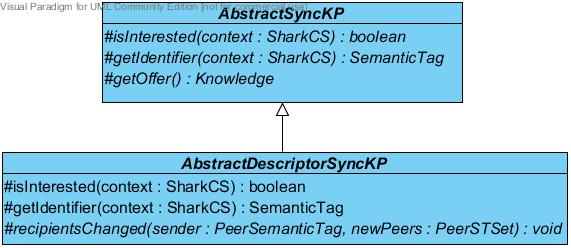
\includegraphics[width=\linewidth]{../Bilder/desc_sync.jpg}
		\caption{Klassendiagramm: AbstractDescriptorSyncKP}
		\label{fig:desc_sync}
	\end{figure}	
	
	Die neue Klasse AbstractDescriptorSyncKP implementiert zwei der drei
	abstrakten Methoden von AbstractSyncKP. Dies bedeutet, dass Entwickler
	nur noch das extrahieren von Wissen übernehmen müssen. Die anderen
	Zwei funktionieren wie folgt:
	
	\begin{itemize}
		\item \textbf{Interesse bekunden:} Weitere Aktionen werden nur ausgeführt,
		wenn der gesendete Deskriptor gleich mit dem von der Klasse gehaltenen
		Deskriptor ist. Gleich bezieht sich hierbei auf die Gleichheit der
		Identifikatoren dieser.
		\item \textbf{Identifikator finden:} Der Identifikator des Knowledge
		Port ist ein künstliches Thema, das in der Topic Dimension des Interesse
		angelegt wurde. Genaueres ist in folgender Erklärung zum 
		künstlichen Interesse beschrieben.
	\end{itemize} 
	
	\paragraph{Nutzung eines künstlichen Interesses}\mbox{} \\
	
	Wie in Abschnitt \ref{sec:artificial_interest} beschrieben wird ein künstliches
	Interesse genutzt. Die Klasse AbstractDescriptorSyncKP baut daher besagtes
	Interesse anhand des übergebenen Deskriptors wie folgt auf. 
	
	\begin{itemize}
		\item \textbf{Topics:} Die Topics Dimension besteht aus einem künstlich
		angelegten Thema. Dieses Thema dient nur dem Zweck Metadaten zu halten.
		\item \textbf{Peers:} Die Peers Dimension einhält den Eigentümer der
		Wissensbasis, auf welchem das Schema zum Deskriptor beruht.
		\item \textbf{Remote Peers:} Die Remote Peers Dimension wird entweder
		vom Konstruktor übernommen (siehe nachfolgende Erläuterung) oder, sollten
		keine Empfänger übergeben worden sein, entspricht sie der Remote Peers
		Dimension des Deskriptor.
		\item \textbf{Direction:} Die Direction Dimension entspricht initial
		immer INOUT. Eine Umschaltung zwischen INOUT und NOTHING ist zu jeder Zeit
		möglich.
	\end{itemize}
	
	Die anderen Dimensionen sind, entsprechend des Konzeptes, leer.
	
	\paragraph{Konstruktoren von AbstractSyncKP und AbstractDescriptorSyncKP}
	\mbox{} \\
	
	In \autoref{fig:desc_sync} sind nicht die Konstruktoren der beiden Klassen
	dargestellt, um Platz im Diagramm zu sparen. Dennoch sind diese von Bedeutung.
	Im folgenden die Parameter für die Konstruktoren der beiden Klassen.
	
	\paragraph{AbstractSyncKP}
	
	\begin{itemize}
		\item \textbf{SharkEngine sharkEngine:} Die SharkEngine, welche von
		dem Port benutzt wird.
		\item \textbf{SyncKB syncKB:} Die Wissensbasis, an der die Zeitstempel
		 gespeichert sind.
		\item \textbf{SharkCS context:} Interesse dieses Ports. Die Remote Peers
		Dimension wird zu Erstellung der Zeitstempel genutzt.
	\end{itemize}
	
	\paragraph{AbstractDescriptorSyncKP}
	
	\begin{itemize}
		\item \textbf{SharkEngine sharkEngine:} Die SharkEngine, welche von
		dem Port benutzt wird. Wird an AbstractSyncKP übergeben.
		\item \textbf{SyncDescriptorSchema schema:} Schema, in welchem sich der
		Deskriptor befindet.
		\item \textbf{ContextSpaceDescriptor descriptor:} Deskriptor, der den
		zu synchronisierenden Datenbereich beschreibt.
		\item \textbf{PeerSTSet recipients:} Personen, mit denen die 
		Synchronisation stattfinden soll.
	\end{itemize}
	
	Zu erkennen ist, dass sich nur ein Parameter gleicht und direkt übergeben 
	werden kann. Aus dem SyncDescriptorSchema kann die SyncKB gelesen und
	übergeben werden. Das künstliche Interesse wird anhand des Schemas, des
	Deskriptors und der Empfänger erstellt und dann ebenfalls dem Konstruktor von
	AbstractSyncKP übergeben. Damit erhält AbstractSyncKP
	dies besagtes Interesse sowie die zum Schema gehörende Wissensbasis.
	
	\paragraph{Besonderheiten von AbstractDescriptorSyncKP}\mbox{} \\
	
	Die Klasse AbstractDescriptorSyncKP weist einige Besonderheiten auf. Zum
	Einen definiert sie zusätzliche Aktionen, zum Anderen haben einige Methoden
	eine besondere Verhaltensweise.
	
	\begin{itemize}
		\item \textbf{Hinzufügen und entfernen von Adressaten:} Eine Änderung
		der Remote Peer Dimension am Interesse der Ports hat keine weiteren
		Aktionen zur folgen. Es müssen die Methoden addRecipient und
		removeRecipient genutzt werden, damit eine Notifikation
		der Änderung an die Kommunikationspartner erfolgt. Die Kindklasse von
		AbstractDescriptorSyncKP muss dabei implementieren, was in diesem
		Fall zu geschehen hat.
		\item \textbf{Änderungen Deskriptoren verteilen:} Es ist möglich, 
		Änderungen des aktuell beschriebenen Deskriptors zu verteilen. Dabei 
		wird der gesamte Baum verteilt und gleiche Deskriptoren beim
		Ziel überschrieben.
		\item \textbf{Getter für den Deskriptor:} Der Getter ließt den 
		Deskriptor direkt aus den Metadaten. Dies bedeutet, er wird aus dem XML
		erstellt. Somit schlagen wirken Änderungen an diesem nicht sofort auf
		den Port aus. Um eine Änderung am Knowledge Port durchzuführen muss der
		Setter aufgerufen werden.
		\item \textbf{Subskription:} Die Methoden subscribe und unsubscribe setzen
		die Direction Dimension des Ports. Ein abonnierter Port wird immer Daten
		versenden und empfangen, währenddessen ein nicht abonnierter Port keine
		Aktionen durchführt.
	\end{itemize}
	
	\subsubsection{Eine Standardimplementierung}
	
	Mit StandardDescriptorSyncKP existiert eine Standardimplementierung, die
	den einfachsten Fall abdeckt. Die beiden noch zu implementierenden
	abstrakten Methoden führen folgende Aktionen aus.
	
	\begin{itemize}
		\item \textbf{Zusammenstellen des Angebotes:} Aus der Wissensbasis
		wird nur das Wissen zum Kontext des im Port gehaltenen Deskriptors
		extrahiert. Jede Art von Beziehungen findet keine Beachtung.
		\item \textbf{Änderung von Adressaten:} Die Remote Peer Dimension 
		wird mit den gesendeten neuen Peers ausgetauscht. Dabei wird
		der Besitzer des Ports, genauer Besitzer des Schemas, welches am Port
		gespeichert ist, mit dem Sender ausgetauscht. Ist der Besitzer ein Teil 
		der neuen Remote Peer Dimension, bedeutetet dies, dass der Sender der
		Nachricht mit diesem kommunizieren möchte. Ist der Besitzer nicht in der
		Liste der neuen Adressaten, möchte der Sender nicht mehr mit diesem Port
		kommunizieren und wird daher aus den Adressaten entfernt.
		\autoref{fig:peer_sync} veranschaulicht den Ablauf noch einmal
		skizzenhaft in einem Aktivitätsdiagramm.
	\end{itemize}
	
	\begin{figure}[H]
		\centerline{
			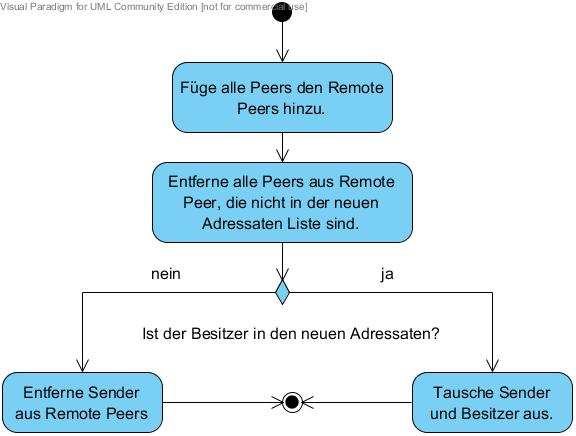
\includegraphics[scale=0.66]{../Bilder/peer_sync.jpg}
		}
		\caption{Skizze: Ablauf der Änderung von Adressaten}
		\label{fig:peer_sync}
	\end{figure}	
		
	\subsection{Ein Knowledge Port zum Lernen von Deskriptoren}
	
	Das Lernen und Lehren von neuen Deskriptoren übernimmt ein Knowledge Port,
	der völlig unabhängig zu den bisher vorgestellten Ports operiert.
	\autoref{fig:assimilation} skizziert die wichtigsten Aspekte der
	zugehörigen Klasse DescriptorAssimilationKP.
	
	\begin{figure}[H]
		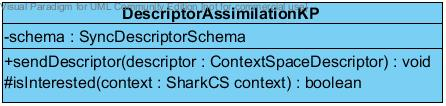
\includegraphics[width=\linewidth]{../Bilder/assimilation.jpg}
		\caption{Klassendiagramm: DescriptorAssimilationKP}
		\label{fig:assimilation}
	\end{figure}	
	
	Die Klasse basiert auf einem Schema. Ein Port kann dabei beliebig viele
	Deskriptoren versenden. Voraussetzung aber ist, dass sie sich so identisch 
	im Schema befinden. Dabei wird nicht der Deskriptoren selbst gesendet sondern
	sein gesamter Baum. Dies ist notwendig, damit auch Beziehungen von 
	Kommunikationspartnern erlernt werden. Die Adressaten fügen den
	Baum dann wie erhalten bei sich ein, wobei bereits existierende Deskriptoren 
	überschrieben werden. Von Interesse ist auch die isInterested Methode. 
	Im Standardfall liefert sie immer true zurück kann aber überschrieben werden,
	um zu unterscheiden, wann ein Baum zu assimilieren ist und wann nicht.
	
	\newpage
	\section{Tests}
	
	Dieses Kapitel widmet sich den Test zur Qualitätssicherung. Es wird beschrieben,
	wie diese sichergestellt wurde.
	
	\subsection{Unit Test und Testabdeckung}
	
	Zur Sicherstellung der Funktionalität der Softwarekomponente wurden Unit Tests
	geschrieben. Da das Projekt ein Maven Projekt ist befinden sich die Tests, nach
	der Konvention, im Verzeichnis src/test/java (siehe \autoref{sec:CD}). Alle
	Test verlaufen ohne Fehler. \\
	
	Des Weiteren wurde Cobertura genutzt um die Testabdeckung zu gewährleisten. \\
	
  	\begin{figure}[H]
		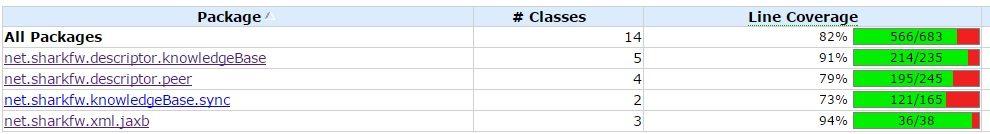
\includegraphics[width=\linewidth]{../Bilder/code.jpg}
		\caption{Ausschnitt: Cobertura Report}
		\label{fig:code}
	\end{figure}	
	
	\autoref{fig:code} zeigt einen Ausschritt des Cobertura Reports. Zu sehen
	ist, dass die Line Coverage immer über 70\% und im Durchschnitt bei 
	83,8\% liegt. Dies wird als ausreichende Testabdeckung betrachtet.
	
	\subsection{Codequalität}
	\label{sec:pmd}
	
	Zur Sicherstellung der Qualität des Quellcodes wurde das Werkzeug PMD genutzt.
	Ein Report dazu kann auf der beiliegenden CD	
	(siehe \autoref{sec:CD}) gefunden werden.
	Genutzt wurde die Standardkonfiguration von PMD. Das heißt, die Regeln definiert
	in basic.xml, unusedcode.xml und imports.xml wurden überprüft. Die einzig
	auffallende Regelverletzung dabei ist \emph{Useless parentheses}. Dabei
	handelt es sich im Code um die Zusammenstellung eines booleschen Ausdrucks.
	Die Klammern dienen der Lesbarkeit. Die \emph{Avoid modifiers which are implied
	by the context} Warnung wird ebenfalls ignoriert, da sie für die Lesbarkeit
	als nicht relevant erachtet wird.
	
	\subsection{Test der Anforderungen }
	Im folgenden ist beschrieben, wie die Funktionalen und nicht funktionalen
	Anforderungen getestet wurden.
	
	\paragraph{Funktionale Anforderungen}
	\begin{itemize}
		\item \textbf{Beschreibbarkeit:} Die Beschreibbarkeit ist durch den
		Deskriptor umgesetzt worden. Es existieren Unit Tests für das Schema
		von Beziehungen. Durch den fehlerfreien Ablauf dieser ist die
		Umsetzung dieser Anforderung gesichert.
		\newpage
		\item \textbf{Beziehungen:} Die Beziehungen wurden durch das Schema
		umgesetzt. Die hier existierenden Unit Tests sichern die Erfüllung
		dieser Anforderung.
		\item \textbf{Persistenz:} Über das Schema können Beschreibungen gespeichert
		und geladen werden. Unit Test beweisen, dass diese Anforderung umgesetzt
		wurde.
		\item \textbf{Synchronisation:} Es wurde ein Klassenkonstrukt geschaffen,
		welches eine Synchronisation auf der Grundlage der entwickelten Deskriptoren
		ermöglicht. Auch hier beweisen Unit Test deren Funktionalität.
		\item \textbf{Änderbarkeit:} Deskriptoren besitzen einen Identifikator über
		den sie Unabhängig von ihrem Kontext auffindbar sind. Somit kann
		eine Änderung ohne Verlust des Deskriptors durchgeführt werden. 
		Beweis hierfür sind Unit Tests des Schemas.
		\item \textbf{Änderung kommunizieren:} Änderungen können über die
		Klassen zur Synchronisation kommuniziert werden. Diese wurden anhand
		von Modultests getestet und daher gilt die Anforderung als umgesetzt.
	\end{itemize} 	
	
	\paragraph{Nicht funktionale Anforderungen}
	\begin{itemize}
		\item \textbf{Build-Management:} Maven wurde als Tool für das
		Build-Management gewählt. Das Projekt konnte in eine Netbeans IDE
		nach dem klonen aus einem Git Repository ohne Probleme importiert werden.
		Des Weiteren ermöglicht die erstellte Konfiguration das Erstellen von
		Cobertura und PMD Reports. 
		\item \textbf{Testbarkeit:} Es existieren Unit Test, daher ist der Quellcode
		testbar.
		\item \textbf{Modultest:} Es wurden eine Reihe von Unit Test geschrieben und
		ein Cobertura Report erstellt.
		\item \textbf{Wartbarkeit:} Der PMD Report erzeugt nur unwesentliche
		Meldungen, die ignoriert werden können (sie Erklärung in Abschnitt
		\ref{sec:pmd}). Von daher kann davon ausgegangen werden, dass der Quellcode
		lesbar ist und somit gewartet werden kann. Für weitere Erklärungen kann
		die JavaDoc Dokumentation (siehe \autoref{sec:CD}) und diese Arbeit selbst
		herangezogen werden.
	\end{itemize} 
	
	\newpage
	\section{Fazit}
	
	In diesem Kapitel soll die Arbeit noch einmal in ihrer Gesamtheit betrachtet
	werden. Zuerst wird kritisch auf Mängel und Verbesserungsmöglichkeiten
	eingegangen. Anschließend folgt das Schlusswort, welches die Ergebnisse 
	bewertet und für zukünftige Projekte einordnet.
	
	\subsection{Mängel und Verbesserungsmöglichkeiten}
	
	Folgend sind die Mängel und Verbesserungsmöglichkeiten der in dieser Arbeit
	entstandenen Softwarekomponente im Detail beschrieben.
	
	\begin{itemize}
		\item \textbf{Keine vollständige Synchronisation in einem Schritt:}
		Es ist nicht gelungen eine vollständige Synchronisation in einem
		einzigen Schritt zu implementieren. Das Ausführen der Aktionen Pull
		und Pull Request führt zwar zum gleichen Ergebnis, erfordert
		aber trotzdem, dass diese einzeln angestoßen werden. Leider ist im
		Shark Framework sowie im Algorithmus der SyncKB, auf dem aufgebaut wurde, 
		nicht klar, wann ein Knowledge Port seine Arbeit beendet hat. Daher erfolgt
		eine vollständige Synchronisation in der entwickelten Softwarekomponente in 
		zwei Schritten.
		\item \textbf{Kein Caching:} Die aktuelle Implementierung des Schemas
		liest die Deskriptoren bei jeden Zugriff aus ihrer persistenten
		Form. Dies können unter Umständen Dateizugriffe sein, was die Laufzeit
		der Aktionen erhöht. Auch die Umwandlung von XML in ein Java Objekt bei
		jedem Zugriff kostet Laufzeit. Ein Caching der Deskriptoren wäre
		anzuraten, sollte der Quellcode einem Refactoring unterzogen werden.
		In dieser Arbeit wurde in erster Linie auf Funktionalität Wert gelegt
		und das Laufzeitproblem deswegen vernachlässigt. 
		\item \textbf{Keine Test von Multithreading:} Die vorhandenen Modultests
		beweisen die Funktionalität der Softwarekomponente nur im kleinen Rahmen.
		Tests mit einer großen Anzahl an Personen, die sich synchronisieren wollen,
		wurden nicht durchgeführt. Das Verhalten in einer Situation dieser Art ist
		also unklar.
		\item \textbf{Komplexität:} Die Nutzung eines künstlichen Interesse
		ist komplex und entspricht nicht dem normalen Vorgehen im Shark
		Framework. Aufgrund der fehlenden Metadaten-Dimension war dies aber
		notwendig. Leider ist somit die interne Funktionsweise der
		Softwarekomponente für Außenstehende schwer zu verstehen. Sollte
		je eine zusätzliche Dimension für Metadaten eingeführt werden, ist
		ein Refactoring des künstlichen Interesses anzuraten.
		\item \textbf{Schema als Sammlung von Bäumen:} Das Schema ist aktuell
		eine Sammlung von Baumstrukturen. Grund hierfür ist, dass die meisten
		Social Media Formate entweder Listen von Einträgen sind oder selbst
		Baumstrukturen besitzen. In dieser Arbeit wurde nicht analysiert,
		welche anderen Formate mit den Deskriptoren dargestellt werden können.
		Es ist möglich, dass in der Zukunft ein Netz oder eine Taxonomie besser 
		geeignet ist, um Beziehungen von Deskriptoren darzustellen.
		\item \textbf{Eliminierung des Piggyback Algorithmus:} Ob die 
		Eliminierung des Piggyback Algorithmus gerechtfertigt war, ist fraglich.
		Gerade bei dem Versand größerer Datenmengen, was hier nicht getestet wurde.
		Das Beheben des aufgetretenen Fehlers hatte Priorität. In zukünftigen
		Anpassungen sollte daher überlegt werden, ob der Piggyback Algorithmus
		wieder eingeführt werden sollte.
		\newpage
		\item \textbf{Trennung von Assimilation und Deskriptoren-Synchronisation:}
		Die Klassen AbstractDescriptorSyncKP und DescriptorAssimilationKP 
		können beide zum Austausch von Deskriptoren genutzt werden. 
		Erstere behandelt nur Deskriptoren, die bereits bei allen
		Kommunikationspartner existieren, währenddessen die Zweite das Erlernen
		dieser ermöglicht. Da sich Algorithmus und Aufbau ähneln ist zu überlegen,
		ob die Klassen vereint werden können.	
	\end{itemize} 
	
	\subsection{Schlusswort}
	
	In dieser Arbeit ist es gelungen einen Algorithmus zu implementieren, der
	es ermöglicht, definierte Bereiche einer Wissensbasis zu synchronisieren.
	Dabei ist eine Beschreibung eines Raumes von Daten die Grundlage. Diese
	ist nicht an die Synchronisation gebunden und kann auch
	für andere Anwendungsfälle genutzt werden. Es besteht die Möglichkeit Beziehungen
	zwischen den Räumen zu definieren. Besagte Beziehungen sind abstrakt und können
	je nach	vorliegendem Fall einem anderen Zweck dienen. Durch Ableitung der 
	Klassen zur Synchronisation ist	es möglich diese anzupassen. Dadurch kann 
	die vorliegende Softwarekomponente auch in Projekten mit
	anderen Anforderungen eingesetzten werden. Allerdings hat die Implementierung
	noch nicht ihre Tauglichkeit für größere Projekte bewiesen. Die 
	durchgeführten Modultests sind klein bezogen auf die Anzahl an Personen
	und Daten. Es ist zu erwarten, dass in Zukunft Probleme auftauchen,
	die in dieser Arbeit nicht aufgegriffen wurden. Von daher stellt die Arbeit
	eher ein Proof of Concept als eine ausgereifte Implementierung dar. 
	Die Wahrscheinlichkeit, dass sich zukünftige Projekte mit der Verfeinerungen 
	der hier beschriebenen Methode und Algorithmen befassen müssen, ist hoch. 
	
	\newpage
	\section{Quellenverzeichnis}	
	
	\printbibliography[type=article,heading=subbibliography,title={Artikel}]
	\printbibliography[type=book,heading=subbibliography,title={Bücher}]
	\printbibliography[type=manual,heading=subbibliography,title={Handbücher}]
	\printbibliography[type=misc,heading=subbibliography,title={Publikationen}] 			\printbibliography[type=report,heading=subbibliography,title={Spezifikationen}]
	\printbibliography[type=online,heading=subbibliography,title={Webseiten}]

	\newpage
	\section{Abbildungsverzeichnis}
	\makeatletter
		\@starttoc{lof}% Print List of Figures
	\makeatother
		
	\newpage	
	\begin{appendix}
	
	\section{CD-ROM zur Arbeit}
	\label{sec:CD}
	
	Die beiliegende CD-ROM zur Arbeit enthält die folgenden Inhalte.
	
	\begin{itemize}
		\item \textbf{Chatprogramm:} Ein ausführbares JAR-Archivmit einem
		Chatprogramm, das die Funktionalität der entwickelten 
		Softwarekomponente beweist. Siehe auch Anhang \ref{sec:chatprogramm}.
		\item \textbf{Dokumentation:} Dieses Verzeichnis unterteilt sich in:
		\begin{itemize}
			\item \textbf{apidocs:} JavDoc Dokumentation.
			\item \textbf{cobertura:} Cobertura Report
			\item \textbf{pmd:} HTML Datei mit einem PMD Report.
		\end{itemize} 
		\item \textbf{Quellcode:} Der Quellcode zu dieser Arbeit
		als ein Maven-Projekt. Das Projekt bringt alle Abhängigkeiten mit
		und kann über den \emph{install} Befehl von Maven gebaut werden. \\
		Weitere Informationen zu maven sind unter \url{https://maven.apache.org/}
		zu finden.	
		\item \textbf{Masterarbeit.pdf:} Diese Arbeit im PDF Format.
	\end{itemize} 
	
	Die Quellen existieren zusätzlich in GitHub unter 
	\url{https://github.com/SharedKnowledge/Incubator/tree/master/Descriptor}. \\
	
	Das Maven Projekt ist konfiguriert eine Cobertura Report über den Maven Befehl 
	\emph{cobertura:cobertura} zu erstellen. Ein PMD Report kann über den Maven
	Befehl \emph{pmd:pmd} erstellt werden.
	
	\newpage
	\section{Systemvoraussetzungen}
	
	Das Projekt wurde konfiguriert um mit folgenden Versionen kompatibel zu sein.	
	
	\begin{itemize}
		\item \textbf{Quellcode:} Java 1.7
		\item \textbf{Compiliert für:} Java 1.7
		\item \textbf{Getestet mit:} Java 1.8
	\end{itemize} 
	
	\newpage
	\section{Chatprogramm}
	\label{sec:chatprogramm}
	
	Im folgenden ist kurz erklärt, wie das Chatprogramm genutzt werden muss.
	
	\begin{figure}[H]
		\centerline{
			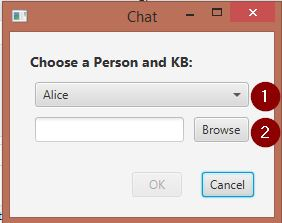
\includegraphics{../Bilder/chat_start.jpg}
		}
		\caption{Start des Chatprogramms}
		\label{fig:chat_start}
	\end{figure}	
	
	\autoref{fig:chat_start} zeigt das Startfenster.
	Über Punkt 1 Kann eine Person gewählt werden, die man darstellt. Punkt
	2 dient der Wahl einer Wissensbasis. Dabei wird in dem gewählten Ordner
	ein Unterordner erstellt, der genauso heißt wie der Peer in Punkt 1. Es
	sollte daher \textbf{nie} der Ordner mit dem Namen der angezeigten Person
	ausgewählt werden, sonder das Verzeichnis in dem dieser liegt.
		
	\begin{figure}[H]
		\centerline{
			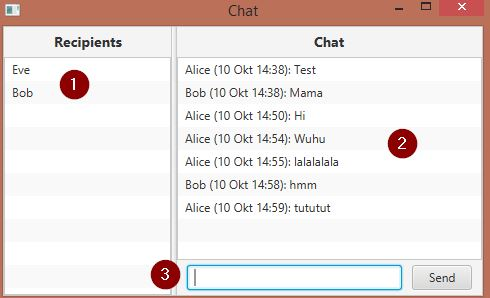
\includegraphics[scale=0.75]{../Bilder/chat_chat.jpg}
		}
		\caption{Chatbereich des Chatprogramms}
		\label{fig:chat_chat}
	\end{figure}	
	
	\autoref{fig:chat_chat} zeigt den Chatbereich. Die Kommunikationspartner
	sind immer die nicht ausgewählte Personen, zu sehen in Punkt 1. Punkt 2
	zeigt den eigentlichen Chat. In das Textfeld in Punkt 3 können die
	Nachrichten eingeben werden. \\
	
	
	Der Chat kommuniziert nur über localhost. daher müssen zwei Instanzen des
	Programms geöffnet werden. Wird zwei mal die gleiche Person gewählt für dies
	zu einem Fehler. Auch das Programm Quick \& Dirty geschrieben. Daher kann es
	zu Verzögerungen beim Start des Chatbereiches und senden von Daten kommen. Zur
	ausgiebigen Nutzungen ist es nicht geeignet sondern stellt ein
	Proof of Concept da.
	

	\newpage	
  	\section{Eigenständigkeitserklärung}
  	Hiermit versichere ich, dass ich die vorliegende Masterarbeit selbstständig und
  	nur unter Verwendung der angegebenen Quellen und Hilfsmittel verfasst habe. Die
  	Arbeit wurde bisher in gleicher oder ähnlicher Form keiner anderen
  	Prüfungsbehörde vorgelegt. \\ \\
  	
 	Datum: \hspace{10pt} Berlin, 12. Oktober 2015 \hspace{30pt} Unterschrift:

	\end{appendix}
  	
\end{document}